
\documentclass[subscriptcorrection,upint,nolists, varvw,barcolor=Goldenrod3,mathalfa=cal=euler,balance,hyphenate,french]{asmejour} %
\let\Bbbk\relax
\usepackage{amsmath,amssymb,amsfonts}
\usepackage{graphicx}
\usepackage{algorithm,algorithmic}
\usepackage{hyperref}
\usepackage{textcomp}
\usepackage{tikz}
\usetikzlibrary{positioning,shapes.geometric,arrows.meta,fit,backgrounds,calc}
\tikzset{
  proc/.style    = {rectangle, rounded corners=2pt, draw=black!70, thick,
                    fill=blue!6, align=center, inner sep=4pt,
                    minimum height=8mm, font=\small},
  term/.style    = {ellipse, draw=black!70, thick, fill=violet!18,
                    align=center, inner sep=3pt, minimum height=8mm, font=\small\bfseries},
  dec/.style     = {diamond, aspect=2.2, draw=black!70, thick, fill=orange!18,
                    align=center, inner sep=1pt, font=\footnotesize},
  state/.style   = {rectangle, rounded corners=6pt, draw=teal!80!black, thick,
                    fill=teal!10, align=center, inner sep=3pt,
                    minimum height=7mm, minimum width=24mm, font=\small},
  io/.style      = {rectangle, draw=black!60, fill=green!8, align=center,
                    font=\scriptsize, inner sep=3pt, minimum height=6mm},
  ext/.style     = {rectangle, rounded corners=2pt, draw=black!70, thick,
                    fill=gray!12, align=center, font=\small, inner sep=4pt,
                    minimum height=9mm},
  lane/.style    = {rectangle, rounded corners=4pt, draw=blue!30, dashed,
                    fill=blue!3, inner sep=6pt},
  flow/.style    = {-{Stealth[length=2.4mm]}, thick, black!75},
  bus/.style     = {{Stealth[length=2.2mm]}-{Stealth[length=2.2mm]}, thick, black!65},
}
\newtheorem{theorem}{Theorem}
\newtheorem{remark}{Remark}

\hypersetup{%
	pdfauthor={John H. Lienhard},
	pdftitle={ASME Journal Paper LaTeX Template},
	pdfkeywords={ASME journal paper, LaTeX template, BibTeX style, asmejour class},% <=== change to YOUR pdf keywords
	pdfsubject = {Describes the asmejour LaTeX template},
	pdflicenseurl={https://ctan.org/pkg/asmejour},% may delete
}

\JourName{Autonomous Vehicles \\ and Systems}%<=== change to the name of your journal

\begin{document}

\SetAuthorBlock{Lovesh Goyal}{Department of Aerospace Engineering,\\
   Indian Institute of Technology Madras,\\
   Chennai, India\\
   email: ae24d401@smail.iitm.ac.in} 

\SetAuthorBlock{Joel George Manathara\CorrespondingAuthor}{%
Associate Professor\\
Department of Aerospace Engineering,\\
Indian Institute of Technology Madras, \\
Chennai, India \\
email: joel@smail.iitm.ac.in
}

\title{Scalable Task Allocation and Airspace
Deconfliction for Mine-Dispensing UAV Swarms, Assignment problem}

\keywords{Multi-UAV operation, Airspace deconfliction, Task allocation, Heuristic algorithm}
   
\begin{abstract}
The autonomous allocation and scheduling of drone swarms in large-scale missions is a computationally challenging problem, as the search space grows rapidly with the number of drones and targets. 
This paper addresses a mine-dispensing problem in which multiple Unmanned Aerial Vehicles (UAVs) transport mines from a base to a set of desired target locations. Each UAV returns to the base after each delivery to collect the next mine.
Since the problem is NP-hard, obtaining exact or near-optimal solutions often results in prohibitive computational time. 
Therefore, we propose heuristic-based algorithms for multi-UAV mission planning that achieve near-optimal mission makespan while significantly reducing computation time, making them suitable for real-world deployment. 
The framework accounts for spatial and temporal deconfliction by incorporating strategies for altitude assignment, sector-based scheduling, and dynamic wait-time adjustments to mitigate mid-air conflicts and overlapping target operations. 
The Simulation results demonstrate that, compared to optimal MILP-based planning, the proposed RRS algorithm reduces computation time by 50 times for missions with more than 20 targets, while maintaining mission makespan within 5\% of optimal, thereby providing a practical and reliable solution.
The approach is further validated through high-fidelity simulations in Gazebo using ROS 2 and PX4-based UAV models, demonstrating its suitability for real-world mine-dispensing operations and extensibility to other large-scale swarm applications.

\end{abstract}

\date{Version \versionno, \today}%% You can modify this information as desired. 

\maketitle

\section{Introduction}
Unmanned Aerial Vehicles (UAVs) are being increasingly employed in various domains, including package delivery \cite{Yang2023, Jin2023}, medical logistics, disaster recovery management \cite{Ijaz2023}, construction site surveillance, and precision agriculture \cite{Qu2022, Alzahrani2020}, where they enhance efficiency while minimizing human effort, time, and cost.
In defense applications, UAVs play a critical role in tasks such as reconnaissance \cite{Zhang2023}, controlled payload deployment, and bomb disposal. 
Their cost-effectiveness, compared to conventional military equipment, has further accelerated their adoption.

Over the past decade, UAV technology has witnessed significant advancements, particularly in swarm systems \cite{Javed2024, Munasinghe2024}, where multiple UAVs operate in coordination to execute complex tasks \cite{Qamar2022, Chen2024, Xia2020}. 
Swarm UAVs offer distinct advantages, including reduced mission time, redundancy, and improved operational flexibility. 
Consequently, research on swarm coordination has expanded substantially, focusing on efficient task allocation and deconfliction strategies \cite{Neville2023, Duan2021}.

One important application of coordinated UAV swarms is the rapid deployment of ground-denial systems over large areas \cite{Reddy2023, Yoo2021}. 
In defense scenarios, thousands of land mines may need to be placed within a short time across geographically distributed target locations. 
Traditional deployment methods rely on manual placement or ground vehicles that disperse mines over a region. Manual placement is slow and labor-intensive, making it unsuitable for large-scale or time-critical missions.
Ground-based dispersal systems, while faster, often release mines without precise positioning.
Such uncontrolled deployment complicates post-mission recovery and increases long-term safety risks due to uncertainty in mine locations.

These limitations motivate the need for controlled, traceable, and precisely planned deployment strategies. 
A coordinated UAV swarm enables parallelized delivery, significantly reducing mission duration. The GPS-referenced aerial deployment ensures accurate placement and digital logging of mine locations, facilitating accountability and potential recovery.
Moreover, swarm systems provide scalability, allowing adaptation to varying mission sizes and mine densities (mines/m$^2$).

However, enabling large-scale UAV swarms introduces significant computational and operational challenges. 
As the number of UAVs and targets increases, the allocation of drones to targets and the scheduling of repeated delivery cycles result in combinatorial growth in possible solutions.
The underlying task allocation problem in land mine deployment using UAV swarms is closely related to classical NP-hard combinatorial problems such as the Vehicle Routing Problem (VRP) \cite{Dorling2017}, the Multiple Traveling Salesman Problem (mTSP) \cite{Assaf2017}, and the Multiprocessor Resource Allocation Problem \cite{Huang2016}.
Since these problems exhibit exponential growth in solution complexity, for missions of practical interest—on the order of hundreds of UAVs and thousands of targets—the computational cost of obtaining exact solutions becomes prohibitive.

In addition to computational complexity, practical multi-UAV missions are constrained by finite operational airspace.
As swarm density increases, ensuring safe spatial and temporal separation among UAVs becomes critical to prevent in-flight conflicts and congestion near the base.

In this work, we focus on a large-scale mine-dispensing mission in which multiple UAVs repeatedly transport mines from a central base to designated target locations within a constrained operational airspace. Each UAV follows a cyclic delivery pattern, returning to the base after each deployment to pick up the next mine to be deployed. 
This paper specifically addresses the resulting large-scale multi-UAV task allocation problem with the objective of producing feasible mission plans within operationally feasible computational times.


% We propose scalable heuristic algorithms integrated with airspace management strategies to ensure safe and efficient execution in dense swarm scenarios. To guarantee safety in dense swarm scenarios, we further introduce a deterministic post-processing conflict-resolution layer based on slack absorption, which fully resolves vertical flight-path intersections without degrading the heuristically optimized mission makespan.
We propose scalable heuristic algorithms integrated with airspace management strategies to ensure safe and efficient execution in dense swarm scenarios. To further guarantee safety, we introduce a post-processing conflict-resolution layer that eliminates residual mid-air conflicts while preserving mission efficiency.

To evaluate our approach, we formulate the complete problem as a Mixed-Integer Linear Programming (MILP) model and solve it in MATLAB, yielding optimal solutions for moderate-sized instances, enabling a quantitative comparison of solutions and computational time with the proposed heuristic algorithms. 
We further validate the proposed planning framework through high-fidelity simulations in Gazebo, integrated with ROS 2 middleware and PX4 Software-In-The-Loop (SITL) flight controllers, enabling realistic closed-loop execution of the planned missions.


The key contributions of this paper are summarized as follows:
\begin{enumerate}
    \item We develop a comprehensive mathematical formulation of the large-scale multi-UAV mine-dispensing problem that jointly incorporates task allocation, cyclic delivery scheduling, and explicit airspace separation constraints within a constrained operational environment.
    
    \item We propose two scalable heuristic algorithms with low time complexity that jointly perform UAV allocation and airspace deconfliction by partitioning the airspace into angular sectors and disjoint vertical layers, ensuring that no two UAVs occupy the same sector--altitude corridor simultaneously.
    
    \item We design a deterministic post-processing conflict-resolution algorithm that utilizes temporal slack absorption. This layer guarantees spatial-temporal deconfliction during vertical flight transitions in congested airspace while strictly preserving the optimized mission makespan.
    \item We formulate the complete problem as a Mixed-Integer Linear Programming (MILP) model that captures all operational constraints and obtain optimal solutions for moderate-sized instances to quantitatively evaluate the performance of the proposed heuristics.
    \item We validate the proposed approach through realistic simulations in Gazebo using ROS 2 and PX4, demonstrating its applicability to real-world scenarios.  

\end{enumerate}

\begin{figure*}[!ht]
    \centering
    \includegraphics[width=\textwidth, height=7cm]{photos/mission scenario.pdf}
    \caption{Mission Scenario}
    \label{fig:mission_scene}
\end{figure*}
.
\section{Problem statement}
We define the Mine–Dispensing Problem (MiDeP)
in a constrained airspace environment, explicitly considering task allocation, scheduling, and airspace deconfliction.

The mission is defined over a rectangular area ($M_A$) of size \(L \times W\) m\(^2\), where \(L\) and \(W\) denote the length and width of the battlefield, respectively. 
Within this region, mines must be deployed at designated target locations. 
These target locations may be either manually specified or generated randomly according to a density parameter \(\rho\) (mines/m\(^2\)) under the assumption of a uniform distribution, as shown in Figure \ref{fig:mission_scene}.

A fleet of \(M\) homogeneous UAVs, 
\[
D=\{d_1, d_2, \dots, d_M\} 
\]
is deployed from a common base station $B$, located at the origin \((0,0)\). Each UAV follows a shuttle-based operation cycle of \emph{Base~\(\rightarrow\)~Target~\(\rightarrow\)~Base}; we refer to each such cycle as a \emph{sortie}, in which a UAV delivers exactly one mine before returning to reload.
The UAVs are assumed to be identical in speed, payload capacity, and endurance. 

To ensure safe operations, the 3D airspace is discretized into collision-free corridors. The mission area, $M_A$, is partitioned angularly into $S$ sectors, and UAVs are allowed to operate at a fixed set of $K$  cruise altitudes. 

\[
A=\{a_1, a_2, \dots, a_K\}
\]
A UAV's position at any time is represented by the triplet \((x, y, a_k)\). 
To prevent in-flight conflicts, no two UAVs are permitted to occupy the same sector-altitude pair simultaneously as depicted in Figure \ref{fig:mission_profile}. 

The objective of the MiDeP is to determine both the allocation of targets to UAVs and a corresponding schedule that satisfies the following conditions:
\begin{enumerate}

    \item Exactly one mine is deployed at every target location
    \item Each UAV carries only one mine per sortie and must return to the base to reload after each deployment
    \item UAVs operate concurrently, but no two UAVs occupy the same sector-altitude combination at any time
    % \item The overall duration of the mission (makespan) is minimized, and the execution order of the assigned tasks for each UAV is not constrained beyond feasibility
    \item The overall mission duration (makespan) is minimized, while each UAV is free to carry out its assigned deliveries in any feasible order
\end{enumerate}

% The Mine–Dispensing Problem (MiDeP) involves allocating targets to multiple drones and determining conflict-free flight schedules that minimize the total mission time. 
% We establish that the MiDeP is NP-hard by reduction from the well-known \emph{Partition} problem.

% \begin{theorem}
% MiDeP is NP-hard
% \end{theorem}

% \begin{proof}
% We prove NP-hardness by reduction from the \emph{Partition} problem, which is known to be NP-complete.

% Consider the decision version of a simplified allocation subproblem of MiDeP, in which routing and airspace constraints are ignored. Given $n$ targets with processing times $\{p_1, p_2, \dots, p_n\}$ and $M$ identical drones, the question is whether the targets can be assigned to the drones such that the maximum load (makespan) does not exceed a given bound $B$.

% Given an instance of a Partition with a multiset 
% $S = \{a_1, a_2, \dots, a_n\}$ 
% and total sum $S_{\text{tot}}$, we construct an instance of the allocation problem as follows:
% set $M = 2$, define $p_i = a_i$ for all $i$, and choose $B = S_{\text{tot}}/2$. This construction is clearly polynomial in the size of the input.

% If the Partition instance admits a subset $S_1 \subset S$ such that
% \[
% \sum_{a_i \in S_1} a_i = S_{\text{tot}}/2,
% \]
% then assigning the corresponding targets to drone~1 and the remaining targets to drone~2 yields a feasible schedule with makespan $B$. Conversely, if such an assignment exists, the targets assigned to one drone form a subset whose total processing time equals $S_{\text{tot}}/2$, yielding a valid partition of $S$. 

% Thus, the allocation subproblem is NP-complete.

% Since this allocation problem is a special case of MiDeP (obtained by removing routing and airspace constraints), and MiDeP generalizes this NP-complete problem, it follows that MiDeP is NP-hard.
% \end{proof}

The Mine–Dispensing Problem (MiDeP) involves allocating targets to multiple drones and determining conflict-free flight schedules that minimize the total mission time. 
We establish that MiDeP is strongly NP-hard by reduction from the \emph{3-Partition} problem.

\begin{theorem}
MiDeP is strongly NP-hard.
\end{theorem}

\begin{proof}
We reduce from \emph{3-Partition}, which is strongly NP-complete. An instance of 3-Partition consists of a multiset $A=\{a_1,a_2,\dots,a_{3M}\}$ of positive integers and a bound $B$ satisfying $\sum_{i=1}^{3M} a_i = MB$ and $B/4 < a_i < B/2$ for every $i$; the question is whether $A$ can be partitioned into $M$ triples, each summing exactly to $B$. The bounds on the $a_i$ force every part of such a partition to contain exactly three elements.

Given such an instance, we construct a \emph{complete} MiDeP instance whose airspace constraints can never be violated, so that feasibility is governed solely by how targets are allocated to drones:
\begin{itemize}
    \item Use $M$ drones and a single cruise altitude.
    \item Create $n=3M$ targets and place each one in a distinct angular sector. Since no two targets share a sector, no two UAVs can ever occupy the same sector--altitude corridor, regardless of their schedule. The deconfliction constraints are therefore satisfied vacuously and no UAV ever incurs a wait.
    \item Choose the radial position of target $i$ so that its round-trip sortie time equals $a_i$. The fixed vertical-transit term common to every sortie is absorbed by a constant rescaling of the $a_i$, which preserves the 3-Partition answer and keeps all magnitudes polynomially bounded.
\end{itemize}
The decision question is whether the targets can be allocated to the $M$ drones so that the makespan does not exceed $B$. This construction is clearly polynomial.

Because each target lies in its own sector and induces no wait, the completion time of a drone equals the sum of the sortie times (i.e., the $a_i$ values) of the targets assigned to it.

\smallskip
\noindent\emph{($\Rightarrow$)} If the 3-Partition instance is a yes-instance, assign the three targets of each triple to a distinct drone. Every drone then carries a load of exactly $B$, so the makespan equals $B$ and the schedule is feasible.

\smallskip
\noindent\emph{($\Leftarrow$)} Conversely, suppose the constructed MiDeP instance admits a schedule with makespan at most $B$. The $M$ drone loads are nonnegative, each at most $B$, and sum to $\sum_i a_i = MB$. Hence every drone load must equal exactly $B$: if any load were strictly below $B$, the loads could not sum to $MB$ without some other load exceeding $B$. Moreover, since $B/4 < a_i < B/2$, a load of exactly $B$ is attainable only with exactly three targets---any two targets sum to less than $B$, while any four sum to more than $B$. Therefore the schedule assigns exactly three targets to each drone, and the resulting triples each sum to $B$, yielding a valid 3-Partition.

The two directions show that the constructed instance is a yes-instance of MiDeP if and only if the original instance is a yes-instance of 3-Partition. Since 3-Partition is strongly NP-complete and the reduction is polynomial with polynomially bounded numbers, MiDeP is strongly NP-hard.
\end{proof}

% \section{Literature Review}

% The multi-UAV task allocation problem has been extensively studied, particularly for logistics, surveillance, and inspection missions. 
% In general, these works aim to assign tasks to UAVs while minimizing mission time or travel costs.

% The structural roots of this problem can be traced back to processor allocation and scheduling in distributed computing systems.
% In these early settings, multiple processors were assigned to tasks under strict resource constraints. 
% For example, \cite{Corbalan2005} studied combinatorial scheduling under resource constraints, while \cite{Li2005} developed allocation algorithms to minimize completion time.
% Although these foundational works share structural similarities with multi-agent assignment, they do not involve the spatial or altitude-based constraints inherent to aerial systems.
   
% As research transitioned to UAVs, early work often focused on distributed coordination and dynamic adaptation. 
% \cite{Duan2020} developed a distributed auction-based algorithm for dynamic task assignment, providing a basis for real-time adaptation. Other research has similarly investigated dynamic task reassignment and replanning under uncertainty to address time-varying environments \cite{Wu2023, Wang2025}.  

% More recently, optimization-based methods and hierarchical frameworks have become widely employed to tackle more complex assignments. Techniques such as Particle Swarm Optimization (PSO), Integer Linear Programming (ILP), and Genetic Algorithms are frequently applied. For instance, \cite{Wen2025} proposed a bilayer framework for urban logistics delivery, while \cite{Yang2025} introduced a two-layer framework combining task assignment with path planning using a hybrid genetic algorithm. 
% Similarly, \cite{Zeng2025} proposed a nested PSO–ILP approach for UAV task assignment. Beyond basic allocation, studies like \cite{He2025} proposed PSO-based algorithms combined with heuristics specifically for path planning during inspection missions.

% In the latest advancements (2025–2026), researchers have begun targeting specific operational bottlenecks like energy limits, collision risks, and computational load. 
% \cite{Zhan2025} developed a mixed-integer programming model for urban UAV fleets that jointly optimizes task assignment, time-window compliance, and battery replacement.
% To manage collision risks, \cite{Lu2025} proposed a two-layer search algorithm that forces UAVs to recalculate their physical flight paths when an urban airspace conflict is detected. 
% Finally, to address computational bottlenecks, \cite{Gan2026} proposed a centrality-driven consensus algorithm that groups drones into clusters, successfully reducing coordination complexity for swarms of up to 150 UAVs.

% Despite these significant advancements, a critical gap remains in the literature. 
% Most existing approaches treat routing and scheduling separately, or they focus on unconstrained airspace.
% While recent methods have improved scalability (e.g., \cite{Gan2026}) or addressed flight path deconfliction (e.g., \cite{Lu2025}), they are generally designed for point-to-point urban logistics or small-scale simulations. 
% They do not simultaneously address massive scalability and explicit 3D airspace deconfliction required for high-density, cyclic delivery missions.

% In our preliminary work \cite{Lovesh2025}, we introduced the foundational formulation of the multi-UAV mine-dispensing problem to begin addressing this gap. 
% That study proposed an initial "Farther Target First" (FTF) heuristic, along with a basic binary integer programming model.
% It utilized an Air Traffic Control-like scheduling approach to assign drones to specific sectors and altitude corridors.
% However, while that framework successfully prevented two UAVs from simultaneously cruising at the exact same sector-altitude combination, it lacked a dedicated deconfliction algorithm to handle mid-air vertical intersections during ascent and descent. 
% Furthermore, the preliminary mathematical model was limited in its ability to benchmark massive-scale, dense swarm deployments.

% To resolve these critical safety and performance limitations, this paper significantly extends our prior framework.
% We propose a full-fledged Mixed-Integer Linear Programming (MILP) formulation that comprehensively captures all operational constraints, introduce three highly scalable heuristic algorithms (DCS, RRS, and FRRS), and integrate a deterministic conflict resolution layer that mathematically guarantees collision-free vertical transitions via temporal slack absorption.

\section{Literature Review}

The mine-dispensing problem brings together three threads that have largely been studied in isolation: combinatorial task allocation, cyclic return-to-base delivery routing, and airspace deconfliction. We review each in turn and show that no existing approach jointly addresses them at the scale and with the airspace structure that dense mine-dispensing missions demand.

The structural roots of the problem lie in processor allocation and scheduling for parallel and distributed computing, where independent tasks are assigned to identical resources so as to minimize the overall completion time, or makespan. Processor-allocation policies that minimize execution time under resource constraints have been developed for distributed computing \cite{Corbalan2005, Li2005}, and makespan-oriented allocation has been studied in the context of mixed-parallel workflow scheduling \cite{Huang2016}. These are classical instances of NP-hard makespan minimization and establish the combinatorial lineage of our allocation subproblem; however, they are purely abstract and carry no notion of spatial position, travel, or airspace occupancy, all of which are central to aerial missions.

Once tasks acquire spatial locations and vehicles must travel to them, the problem becomes one of routing. The mine-dispensing mission, in which each UAV repeatedly departs from and returns to a single base, is most closely related to multi-trip vehicle routing and multiple-depot traveling-salesman formulations \cite{Assaf2017}. Multi-trip vehicle routing problems for drone delivery that minimize cost or delivery time while explicitly modeling battery and payload limits have been proposed \cite{Dorling2017}. Closer to our cyclic setting, rooftop parcel delivery in which drones return to a depot to reload after each delivery \cite{Kim2020} and a pickup-to-delivery drone routing problem with an explicit return-to-base constraint \cite{GomezLagos2022} have been formulated as mixed-integer programs solved with makespan-minimizing heuristics. Greedy heuristics for multi-drone package delivery have similarly been benchmarked against optimal solutions \cite{BettiSorbelli2022}. These works confirm the relevance of makespan minimization and the practice of benchmarking heuristics against exact formulations, but they assume free, idealized airspace and are validated only on small to moderate fleets; none enforces spatial--temporal separation among concurrently operating UAVs.

For multi-UAV systems specifically, a large body of work develops allocation and planning methods based on market mechanisms and metaheuristics. An auction-based algorithm has been proposed for distributed task assignment \cite{Duan2020}, while recent frameworks couple assignment with path planning through layered optimization. Bi-level architectures that combine genetic and particle-swarm optimizers have been applied to urban delivery \cite{Wen2025, Yang2025}, and nested particle-swarm and integer-linear-programming layers have been used for swarm task allocation \cite{Zeng2025}. To improve scalability, a clustered consensus-based bundle algorithm reduces coordination overhead for swarms of up to 150 UAVs \cite{Gan2026}. These methods advance solution quality and, in some cases, scale; yet they target point-to-point urban logistics, do not model the cyclic shuttle structure of mine dispensing, and treat the airspace as an unconstrained medium in which any number of vehicles may share the same volume.

A separate line of research addresses the airspace itself. UAS traffic-management studies structure low-altitude airspace into sectors, lanes, and stacked altitude corridors to keep concurrent traffic separated \cite{Lee2023}, mirroring the sector--altitude discretization we adopt. At the planning level, a conflict-free 3D path-planning method detects and resolves inter-UAV conflicts for dense urban operations \cite{Lu2025}, and scheduling and path planning have been jointly optimized under energy and airspace constraints \cite{Zhan2025}. While these works introduce explicit deconfliction, they operate at the level of individual flight paths in grid or corridor maps and are demonstrated on limited problem sizes; they neither minimize a fleet-wide makespan for cyclic delivery nor resolve the mid-air conflicts that arise specifically during vertical ascent and descent between altitude layers.

Taken together, the reviewed literature treats allocation, cyclic routing, and airspace deconfliction largely in isolation: makespan-oriented delivery models ignore airspace separation, scalable allocation methods assume an unconstrained medium, and conflict-free planners are restricted to moderate fleets and do not target cyclic, return-to-base missions. Consequently, no existing approach simultaneously delivers (i) scalability to thousands of targets and hundreds of UAVs, (ii) a cyclic base--target--base delivery structure, (iii) explicit sector--altitude corridor deconfliction, and (iv) minimization of the overall mission makespan.

In our preliminary work \cite{Lovesh2025}, we introduced the mine-dispensing problem and a first solution aimed at closing this gap. That study proposed a Farthest Target First heuristic for allocation, benchmarked against an optimal Integer Linear Programming formulation, together with an air-traffic-control-like scheme that assigns UAVs to sector--altitude corridors. However, while that framework prevented two UAVs from cruising in the same sector--altitude corridor simultaneously, it provided no mechanism to resolve mid-air conflicts during vertical ascent and descent, and its formulation could not benchmark dense, large-scale deployments.

This paper substantially extends that framework along three directions. We develop a complete Mixed-Integer Linear Programming formulation that jointly captures allocation, scheduling, and sector--altitude separation; we propose three scalable heuristic algorithms for combined allocation and deconfliction; and we introduce a deterministic conflict-resolution layer that guarantees collision-free vertical transitions through temporal slack absorption. We further validate the resulting plans in high-fidelity ROS\,2 and PX4 simulations.



\begin{figure*}[!ht]
    \centering
    \includegraphics[width=\textwidth, height=7cm]{photos/mission_profile.pdf}
    \caption{Mission profile}
    \label{fig:mission_profile}
\end{figure*}

% \section{Optimal Problem Formulation}
% \label{sec:optform}

% The Mine–Dispensing Problem (MiDeP) is formulated as a Mixed-Integer Linear Programming (MILP) problem with the objective of minimizing the total mission completion time (\(T_{\max}\)) while ensuring spatial and temporal deconfliction among drones operating in a constrained airspace.

% \subsection{Decision Variables}
% \begin{itemize}
%     \item \(x_{ijk} \in \{0,1\}\): binary variable, equal to 1 if drone \(i\) is assigned to target \(j\) at altitude level \(a_k\), and 0 otherwise.
%     \item \(S_j \ge 0\): continuous variable denoting the start time of mission corresponding to target \(j\).
%     \item \(T_{\max} \ge 0\): continuous variable representing the overall mission completion time (makespan).
%     \item \(u_{i,ab} \in \{0,1\}\): ordering variable indicating the sequence of jobs executed by the same drone; \(u_{i,ab}=1\) if job \(a\) is performed after \(b\) by drone \(i\), and \(0\) otherwise.
%     \item \(y_{abk} \in \{0,1\}\): ordering variable for deconfliction at the same altitude; \(y_{abk}=1\) if job \(a\) is performed after \(b\) at altitude level \(a_k\), and \(0\) otherwise.
% \end{itemize}

% \subsection{Parameters}
% \begin{itemize}
%     \item \(p_{jk}\): mission duration for target \(j\) when assigned to altitude \(a_k\), including climb, cruise, descent, and return times.
%     \item \(\beta_{jk}\): sector cruise occupancy duration of target \(j\) at altitude \(a_k\), representing the time window during which the drone occupies a particular sector–altitude corridor.
%     \item \(st(j)\): sector index corresponding to the spatial location of target \(j\).
%     \item \(M\): sufficiently large positive constant (big-M) used to relax constraints when sequencing conditions are inactive.
%     \item \(m, n, K\): total number of drones, targets, and available altitude levels, respectively.
% \end{itemize}

% \subsection{Objective Function}
% The objective is to minimize the overall mission makespan:
% \begin{equation}
%     \min T_{\max}.
% \end{equation}

% \subsection{Constraints}

% \subsubsection{Task Assignment}
% Each target must be visited exactly once by a single drone at a single altitude level:
% \begin{equation}
%     \sum_{i=1}^{m} \sum_{k=1}^{K} x_{ijk} = 1, \quad \forall j.
% \end{equation}

% \subsubsection{Makespan Bound}
% For each target, the completion time must not exceed the overall makespan:
% \begin{equation}
%     S_j + \sum_{i=1}^{m} \sum_{k=1}^{K} p_{jk}x_{ijk} \le T_{\max}, \quad \forall j.
% \end{equation}

% \subsubsection{No-Overlap on Same Drone}
% For every drone \(i\) and every unordered pair of distinct targets \(a,b\), the operations must be temporally ordered to prevent overlap:
% \begin{align}
%     S_a &\ge S_b + \sum_{k=1}^{K} p_{bk}x_{ibk} - M[1 - u_{i,ab}+2-w_{ai}-w_{bi}], \\
%     S_b &\ge S_a + \sum_{k=1}^{K} p_{ak}x_{iak} - M [u_{i,ab}+2-w_{ai}-w_{bi}].
% \end{align}
% where  \(w_{ji} = \sum_{k=1}^{K} x_{ijk}\) indicates whether target \(j\) is assigned to drone \(i\). These constraints are active only when both targets \(a\) and \(b\) are assigned same drone \(i\).
% If \(u_{i,ab}=0\), task \(a\) precedes task \(b\); if \(u_{i,ab}=1\), the order is reversed.

% \subsubsection{Sector–Altitude Deconfliction}
% For any pair of distinct targets \(a,b\) belonging to the same sector \((st(a)=st(b))\) and any altitude level \(a_k\), two drones cannot simultaneously occupy the same sector–altitude combination:
% \begin{align}
%     S_a &\ge S_b + \beta_{bk} - M[1 - y_{abk} + 2 - z_{ak} - z_{bk}], \\
%     S_b &\ge S_a + \beta_{ak} - M[y_{abk} + 2 - z_{ak} - z_{bk}],
% \end{align}
% where \(z_{jk} = \sum_{i=1}^{m} x_{ijk}\) indicates whether target \(j\) is being serviced at altitude \(a_k\).  
% These constraints are activated only when both targets share the same sector and altitude level; otherwise, they are relaxed.

\section{Optimal Problem Formulation}
\label{sec:optform}

The Mine–Dispensing Problem (MiDeP) is formulated as a Mixed-Integer Linear Programming (MILP) problem with the objective of minimizing the total mission completion time (\(T_{\max}\)) while ensuring spatial and temporal deconfliction among drones operating in a constrained airspace.

\subsection{Parameters}
\begin{itemize}
    \item \(p_{jk}\): sortie duration for target \(j\) when served at altitude \(a_k\), including climb, cruise, descent, and return times. 
    % A sortie reserves its sector--altitude corridor for this entire duration, so \(p_{jk}\) also serves as the corridor-occupancy window.
    \item \(st(j)\): sector index corresponding to the spatial location of target \(j\).
    \item \(M\): sufficiently large positive constant (big-M) used to relax constraints when sequencing conditions are inactive.
    \item \(m, n, K\): total number of drones, targets, and available altitude levels, respectively.
\end{itemize}


\subsection{Decision Variables}
\begin{itemize}
    \item \(x_{ijk} \in \{0,1\}\): binary variable, equal to 1 if drone \(i\) is assigned to target \(j\) at altitude level \(a_k\), and 0 otherwise.
    \item \(S_j \ge 0\): continuous variable denoting the start time of the sortie serving target \(j\).
    \item \(T_{\max} \ge 0\): continuous variable representing the overall mission completion time (makespan).
    \item \(u_{i,ab} \in \{0,1\}\): ordering variable indicating the sequence of jobs executed by the same drone; \(u_{i,ab}=1\) if job \(a\) is performed after \(b\) by drone \(i\), and \(0\) otherwise.
    \item \(y_{abk} \in \{0,1\}\): ordering variable for sector--altitude deconfliction, introduced only for pairs of targets \(a,b\) lying in the same sector (\(st(a)=st(b)\)); \(y_{abk}=1\) if job \(a\) is performed after \(b\) at altitude level \(a_k\), and \(0\) otherwise.
    %  Targets in different sectors can never occupy the same sector--altitude corridor, so no such variable (and no associated deconfliction constraint) is created for them; the sector is thus implied by the pair, and no separate sector index is required.
\end{itemize}



\subsection{Objective Function}
The objective is to minimize the overall mission makespan:
\begin{equation}
    \min T_{\max}.
\end{equation}

\subsection{Constraints}

\subsubsection{Task Assignment}
Each target must be visited exactly once by a single drone at a single altitude level:
\begin{equation}
    \sum_{i=1}^{m} \sum_{k=1}^{K} x_{ijk} = 1, \quad \forall j.
\end{equation}

\subsubsection{Makespan Bound}
For each target, the completion time must not exceed the overall makespan:
\begin{equation}
    S_j + \sum_{i=1}^{m} \sum_{k=1}^{K} p_{jk}x_{ijk} \le T_{\max}, \quad \forall j.
\end{equation}

\subsubsection{No-Overlap on Same Drone}
For every drone \(i\) and every unordered pair of distinct targets \(a,b\), the operations must be temporally ordered to prevent overlap:
\begin{align}
    S_a &\ge S_b + \sum_{k=1}^{K} p_{bk}x_{ibk} - M[1 - u_{i,ab}+2-w_{ai}-w_{bi}], \\
    S_b &\ge S_a + \sum_{k=1}^{K} p_{ak}x_{iak} - M [u_{i,ab}+2-w_{ai}-w_{bi}].
\end{align}
where  \(w_{ji} = \sum_{k=1}^{K} x_{ijk}\) indicates whether target \(j\) is assigned to drone \(i\). These constraints are active only when both targets \(a\) and \(b\) are assigned same drone \(i\).
If \(u_{i,ab}=0\), task \(a\) precedes task \(b\); if \(u_{i,ab}=1\), the order is reversed.

\subsubsection{Sector–Altitude Deconfliction}
For any pair of distinct targets \(a,b\) belonging to the same sector \((st(a)=st(b))\) and any altitude level \(a_k\), two drones cannot simultaneously occupy the same sector–altitude combination:
\begin{align}
    S_a &\ge S_b + p_{bk} - M[1 - y_{abk} + 2 - z_{ak} - z_{bk}], \\
    S_b &\ge S_a + p_{ak} - M[y_{abk} + 2 - z_{ak} - z_{bk}],
\end{align}
where \(z_{jk} = \sum_{i=1}^{m} x_{ijk}\) indicates whether target \(j\) is being serviced at altitude \(a_k\).  
These constraints are activated only when both targets share the same sector and altitude level; otherwise, they are relaxed.



% The formulation jointly captures task allocation, temporal scheduling, and spatial deconfliction within a single optimization framework.  
% Constraint (2) ensures mission completeness, while Constraint (3) guarantees time consistency and limits mission duration.  
% Constraints (4)–(5) enforce mutual exclusivity in drone operations, and (6)–(7) maintain safety through sector–altitude separation.  
% The big-M formulation allows flexible activation of sequencing relations without compromising linearity.  
% The resulting MILP can be solved, for example, using \texttt{intlinprog} in MATLAB, to obtain the optimal makespan and assignment schedule. 


The formulation jointly captures task allocation, temporal scheduling, and spatial deconfliction within a single optimization framework.
Constraint (2) ensures mission completeness, as every target is served exactly once.
Constraint (3) defines the makespan \(T_{\max}\) as an upper bound on the completion time of every target, so that minimizing \(T_{\max}\) minimizes the time at which the last delivery is completed.
Constraints (4)–(5) ensure that each drone performs only one sortie at a time, i.e., the missions assigned to the same drone do not overlap in time, while Constraints (6)–(7) preserve safety by temporally separating any two missions that share the same sector and altitude.
Constraints (4)–(7) are disjunctive: the big-M terms relax a constraint when its governing binary conditions are inactive (the two targets are not assigned to the same drone, or are not flown at the same sector–altitude) and enforce it otherwise, following the standard big-M reformulation of disjunctive sequencing constraints \cite{Manne1960}.
The resulting MILP can be solved, for example, using \texttt{intlinprog} in MATLAB, to obtain the optimal makespan and assignment schedule.





% \section{Proposed Algorithms}


% Once the optimal problem is formulated and given that it is NP-hard, exact methods have exponential time complexity.
% In this section, we propose three heuristic algorithms. 

\section{Proposed Algorithms}

Since the MILP formulation of MiDeP is NP-hard, exact solvers become computationally prohibitive owing to their exponential worst-case time complexity. In this section, we therefore propose two heuristic algorithms that produce feasible schedules in polynomial time.




\subsection{Descending Cost Scheduling (DCS) Algorithm}

 
% The central idea is to minimize the mission completion time by allocating longer missions (farther targets) earlier, while simultaneously ensuring altitude--sector deconfliction. 
% The mission cost is defined as the round-trip distance from the base. 





% As shown in Algorithm~\ref{alg:DCS}, the readiness of all drones and sector–altitude pairs is initialized to zero (Lines~4–5), ensuring that no vehicle or airspace segment is initially occupied.
% Each target $T_j$ is then assigned a sector index $s_j$ and a cost value, representing the round-trip distance from the base (Line~6).
% Targets are sorted in descending order of cost (Line~7), such that distant targets are prioritized for early allocation.


% For each target in this sorted list (Line~8), the algorithm evaluates all possible combinations of drone $i$ and altitude level $a_k$ (Lines~9–17). 
% The earliest feasible start time is computed as the maximum of the drone’s availability and the readiness of the corresponding sector–altitude slot (Line~11). 
% The total flight duration $t_j$ includes vertical and horizontal travel (Line~13).
% The corresponding finish time is then obtained as the sum of the start time and the flight duration (Line~14).
% The combination yielding the smallest finish time is selected as the optimal assignment for that target (Lines~15–17).

% Once the best assignment $(i^\ast, k^\ast)$ is identified, the algorithm computes the drone’s waiting time before departure (Line~21), appends the target, altitude, and wait time—to the drone’s schedule $\mathcal{A}_{i^\ast}$ (Line~22), and updates both drone and sector readiness states (Lines~23–24). After all targets are processed, the overall mission completion time $T_{\mathit{mission}}$ is set to the maximum readiness value across all drones (Line~26).

% In summary, DCS combines a \textit{descending-cost priority} with a \textit{greedy earliest-finish} assignment, producing an efficient heuristic that favors farthest-target-first scheduling while maintaining concurrency through altitude–sector coordination.
% Although greedy, DCS effectively approximates the optimal solution and serves as a strong baseline for more integrated heuristics.

The first heuristic, termed the \emph{Descending Cost Scheduling (DCS)} algorithm, follows a greedy priority-based 
assignment scheme. 
The central idea is to minimize the overall mission makespan by scheduling the longest sorties (those serving the farthest targets) first, while simultaneously ensuring altitude--sector deconfliction.
The cost of a sortie is defined as its round-trip distance from the base.

Algorithm~\ref{alg:DCS} summarizes the DCS procedure: given the target locations, base, fleet size, altitude levels, and sectors, for each drone, it returns an ordered list of sorties (with their targets, altitudes, and wait times) together with the resulting mission makespan $T_{\mathit{mission}}$.
The readiness of all drones and sector–altitude pairs is initialized to zero (Lines~4–5), so that no vehicle or airspace corridor is initially occupied.
For each target $T_j$, its sector index $s_j$ and round-trip cost $c_j$ are computed from the target location (Line~6).
The targets are then sorted in descending order of cost (Line~7), so that farther targets are prioritized for early scheduling.



\begin{algorithm}[H]
\caption{Descending Cost Scheduling (DCS) Algorithm}
\begin{algorithmic}[1]
\STATE \textbf{Input:} Target positions $T_j$, base $B$, number of drones $M$, altitudes $a_k$, sectors $1,\ldots,S$, cruise speed $v_c$, ascent/descent speed $v_v$
\STATE \textbf{Output:} Assignment for $d_i$: $\mathcal{A}_i$ with targets, altitudes, and wait times; $T_{\mathit{mission}} = \max_{i} \mathit{droneReady}_{i}$
\STATE \textbf{Procedure:}
\STATE $\mathit{droneReady}_i = 0$, $\mathcal{A}_i \leftarrow \emptyset$, $\forall i$
\STATE $\mathit{sectorReady}_{sk} = 0$, $\forall s,k$
\STATE $s_j = \text{sectorOf}(T_j)$, $c_j = 2\cdot\|T_j - B\|_2$, $\forall j$
\STATE $\mathcal{T} \gets \text{sortDescending}(T_j \text{ by } c_j)$
\FOR{$T_j$ in $\mathcal{T}$}
    \STATE $bestMakespan \gets \infty$
    \FOR{$i = 1$ to $M$} 
        \FOR{$k = 1$ to $K$} 
            \STATE $startTime \gets \max(\mathit{droneReady}_i,
            \mathit{sectorReady}_{s_jk})$
            \STATE $t_j \gets 4 \cdot {a_k}/v_v + 2 \cdot c_j/v_c$
            \STATE $finishTime \gets startTime + t_j$
            \IF{$finishTime < bestMakespan$}
                \STATE $bestMakespan \gets finishTime$
                \STATE $(i^\ast, k^\ast, startTime^\ast, finishTime^\ast) \gets (i, k, startTime, finishTime)$
            \ENDIF
        \ENDFOR   
        
    \ENDFOR
    \STATE $waitTime \gets startTime^\ast - \mathit{droneReady}_{i^\ast}$
    \STATE appendTo($\mathcal{A}_{i^\ast}, (T_j, a_{k^\ast}, waitTime)$)
    \STATE $\mathit{droneReady}_{i^\ast} \gets finishTime^\ast$
    \STATE $\mathit{sectorReady}_{s_jk^\ast} \gets finishTime^\ast$
\ENDFOR
\STATE $T_{\mathit{mission}} = \max_i \mathit{droneReady}_i$
\end{algorithmic}
\label{alg:DCS}
\end{algorithm}


For each target in this sorted list (Line~8), the algorithm evaluates all possible combinations of drone $i$ and altitude level $a_k$ (Lines~9–17). 
The earliest feasible start time is computed as the maximum of the drone’s availability and the readiness of the corresponding sector–altitude slot (Line~11). 
The total flight duration $t_j$ includes vertical and horizontal travel (Line~13).
The corresponding finish time is then obtained as the sum of the start time and the flight duration (Line~14).
The combination yielding the smallest finish time is selected as the best $(i,k)$ pair for that target (Lines~15–17).

Having identified the best drone–altitude pair $(i^\ast, k^\ast)$ for the current target, the algorithm records the sortie: it computes the wait time the chosen drone incurs before departure (the gap between its readiness and the sortie's start time, Line~21), appends the target, its altitude, and this wait time to that drone's schedule $\mathcal{A}_{i^\ast}$ (Line~22), and advances both the drone's readiness and the sector–altitude corridor's readiness to the sortie's finish time (Lines~23–24). Once every target has been scheduled, the mission makespan $T_{\mathit{mission}}$ is the latest drone readiness across the fleet (Line~26).

In summary, DCS combines a \textit{highest-cost-first priority} with a \textit{greedy earliest-finish} assignment, favoring farthest-target-first scheduling while ensuring parallel drone operations through altitude–sector coordination.
Sorting the targets takes $O(N\log N)$ time, and scheduling each of the $N$ targets evaluates all $M$ drones and $K$ altitudes, so DCS runs in $O(N\log N + NMK)$ time.
Although greedy, DCS provides a fast, scalable baseline; its makespan is benchmarked against RRS and the optimal MILP solution in the performance evaluation.



\subsection{Round-Robin Scheduling (RRS) Algorithm}

% Unlike DCS, which prioritizes distant targets first, the \emph{Round-Robin Scheduling (RRS)} heuristic enforces fairness among drones by cyclically distributing targets in a rotational sequence. 
% This ensures balanced utilization of the fleet, particularly when mission distances or sector distributions are highly heterogeneous. 

% As shown in Algorithm~\ref{alg:RRS}, each target $T_j$ is assigned a sector $s_j$ and cruise distance $c_j$ (Line~6).
% The targets are sorted in descending order of $c_j$  (Line~7), maintaining the same priority order as DCS but with different allocation logic. 
% A drone index counter, $\mathit{droneTurn}$, is initialized (Line~8) and incremented cyclically after each assignment (Line~25).
% For every target (Lines~9–25), the current drone $d_i$ is assigned the next available mission in sequence (Line~10). 
% For this drone, the algorithm iterates through all possible altitudes (Lines~11–18) and selects the one that minimizes the resulting makespan.
% The start time (Line~13) ensures that the drone and the corresponding sector–altitude pair are both available. The total mission duration $t_j$ (Line~14) follows the same flight time model as DCS. 
% The best altitude $a_{k^\ast}$ is chosen by comparing the predicted finish time (Line~16) against the current best makespan (Line~17). 
% Once selected, the wait time and all readiness variables are updated (Lines~21–22), and the round-robin pointer moves to the next drone (Line~25).
% This rotation-based assignment ensures uniform drone load distribution and prevents any single drone from being overutilized, unlike purely greedy methods.
% However, the rigid sequencing may result in slightly longer overall makespans than DCS when the targets are highly asymmetric.


The \emph{Round-Robin Scheduling (RRS)} heuristic targets the main computational cost of DCS. For every target, DCS searches over all $M$ drones to find the earliest-finishing one, which becomes expensive as the fleet grows. RRS sorts the targets by descending cost exactly as DCS does, but instead of searching all drones, it assigns each successive target to the next drone in a fixed cyclic rotation, optimizing only the altitude for that drone. Because the cost-sorted targets are dealt out in rotation, every drone receives an interleaved mix of far and near sorties, so the fleet load stays balanced without an explicit per-target search over drones.

As shown in Algorithm~\ref{alg:RRS}, each target $T_j$ is assigned a sector $s_j$ and cruise distance $c_j$ (Line~6).
The targets are sorted in descending order of $c_j$  (Line~7), maintaining the same priority order as DCS but with different allocation logic. 
A drone index counter, $\mathit{droneTurn}$, is initialized (Line~8) and incremented cyclically after each assignment (Line~25).
For every target (Lines~9–25), the current drone $d_i$ is assigned the next sortie in the rotation (Line~10).
For this drone, the algorithm iterates through all possible altitudes (Lines~11–18) and selects the one that minimizes the resulting makespan.
The start time (Line~13) ensures that the drone and the corresponding sector–altitude pair are both available. The total sortie duration $t_j$ (Line~14) follows the same flight time model as DCS.
The best altitude $a_{k^\ast}$ is chosen by comparing the predicted finish time (Line~16) against the current best makespan (Line~17). 
Once selected, the wait time and all readiness variables are updated (Lines~21–22), and the round-robin pointer moves to the next drone (Line~25).
The advantage of RRS is twofold. Computationally, replacing the search over all $M$ drones with a single rotation step schedules each target in $O(K)$ rather than $O(MK)$ time, giving an overall complexity of $O(N\log N + NK)$ that is independent of the fleet size in the inner loop. In terms of solution quality, the balanced round-robin dealing of the cost-sorted targets avoids the myopic, locally greedy commitments that DCS makes when it fixes each target to its earliest-finishing drone, which can compound into a larger makespan as the problem scales. 


\begin{algorithm}[H]
\caption{Round-Robin Scheduling (RRS) Algorithm}
\begin{algorithmic}[1]
\STATE \textbf{Input:} Target positions $T_j$, base $B$, number of drones $M$, altitudes $a_k$, sectors $1,\ldots,S$, cruise speed $v_c$, ascent/descent speed $v_v$

\STATE \textbf{Output:} Assignment for each drone $d_i$: $\mathcal{A}_i$ with targets, altitudes, and wait times; $T_{\mathit{mission}} = \max_i \mathit{droneReady}_i$
\STATE \textbf{Procedure:}
\STATE $\mathit{droneReady}_i = 0$, $\mathcal{A}_i \leftarrow \emptyset$, $\forall i$
\STATE $\mathit{sectorReady}_{sk} = 0$, $\forall s,k$
\STATE $s_j = \text{sectorOf}(T_j)$, $c_j = 2\cdot\|T_j - B\|_2$, $\forall j$
\STATE $\mathcal{T} \gets \text{sortDescending}(T_j \text{ by } c_j)$
\STATE $droneTurn \gets 1$
\FOR{$T_j$ in $\mathcal{T}$}
    \STATE $i \gets droneTurn$
    \STATE $bestMakespan \gets \infty$
    \FOR{$k = 1$ to $K$} 
        \STATE $startTime \gets \max(\mathit{droneReady}_i, \mathit{sectorReady}_{s_jk})$
        \STATE $t_j \gets 4\cdot a_k/v_v + 2\cdot c_j/v_c$
        \STATE $finishTime \gets startTime + t_j$
        \IF{$finishTime < bestMakespan$}
            \STATE $(k^\ast, startTime^\ast, finishTime^\ast) \gets (k, startTime, finishTime)$
            \STATE $bestMakespan \gets finishTime$
        \ENDIF
    \ENDFOR
    \STATE $waitTime \gets startTime^\ast - \mathit{droneReady}_i$
    \STATE appendTo($\mathcal{A}_i, (T_j, a_{k^\ast}, waitTime)$)
    \STATE $\mathit{droneReady}_i \gets finishTime^\ast$
    \STATE $\mathit{sectorReady}_{s_jk^\ast} \gets finishTime^\ast$
    \STATE $droneTurn \gets (droneTurn \bmod M) + 1$
\ENDFOR
\STATE $T_{\mathit{mission}} = \max_i \mathit{droneReady}_i$

\end{algorithmic}
\label{alg:RRS}
\end{algorithm}




% The Flexible Round Robin Scheduling (FRRS) algorithm builds upon the RRS strategy by relaxing the strict cyclic assignment order.  
% While the Round Robin Scheduling (RRS) algorithm ensures fair distribution by assigning targets to drones in a fixed rotation, it can lead to idle waiting if the next drone in sequence is occupied.  
% FRRS mitigates this by introducing a lightweight adaptive mechanism that searches ahead in the rotation to find an available drone, thereby reducing waiting times and improving concurrency.  
% Thus, FRRS represents a hybrid between the fairness of RRS and the efficiency of cost-driven approaches like DCS.






% As shown in Algorithm~\ref{alg:FRRS}, FRRS begins with the same initialization as RRS (Lines~4–6), setting all drones and sector–altitude pairs to be initially available.  
% Targets are again sorted in descending order of round-trip cost $c_j$ (Line~7) to maintain load balance across drones.

% A rotation pointer $\mathit{nextDrone}$ (Line~8) tracks the next drone to receive an assignment.  
% However, unlike RRS, where the assignment strictly follows this pointer, FRRS explores additional drones with an increasing offset (Lines~10–11).  
% For each candidate drone $i$ and altitude level $a_k$, the algorithm computes the feasible start time (Line~14), mission duration $t_j$ (Line~15), and corresponding finish time (Line~16).  
% It then evaluates the resulting mission makespan (Line~17-18) and retains the assignment that minimizes the overall mission completion time.  
% If two assignments yield the same makespan, the one with a smaller start time is preferred (Line~17).

% Once the best assignment is determined, the algorithm updates the corresponding drone’s availability (Line~23), the sector–altitude occupancy (Line~24), and the rotation pointer (Line~25).  
% This ensures fairness while avoiding excessive idle waiting caused by blocked drones.

% Overall, FRRS preserves the equitable nature of round-robin assignment while improving efficiency by allowing flexible drone selection, resulting in reduced waiting times and a smaller overall makespan than RRS.


\iffalse

\subsection{Flexible Round Robin Scheduling (FRRS)}
The Flexible Round Robin Scheduling (FRRS) algorithm builds upon RRS by relaxing its strict cyclic assignment order.
While RRS assigns each target to the single next drone in the rotation, that drone may be busy, forcing a long idle wait before the sortie can start.
FRRS removes this rigidity: starting from the rotation pointer, it considers every drone and selects the drone--altitude pair that minimizes the makespan, preferring the smaller start time on ties so as to reduce idle waiting.
Because it examines all drones, FRRS does not save computation relative to DCS---both run in $O(N\log N + NMK)$ time. Rather, it combines DCS-style flexible drone selection with RRS's round-robin pointer, which biases the search start and the tie-breaking toward an even rotation across the fleet.

As shown in Algorithm~\ref{alg:FRRS}, FRRS begins with the same initialization as RRS (Lines~4–6), setting all drones and sector–altitude pairs to be initially available.  
Targets are again sorted in descending order of round-trip cost $c_j$ (Line~7) to maintain load balance across drones.

A rotation pointer $\mathit{nextDrone}$ (Line~8) tracks the next drone to receive an assignment.  
However, unlike RRS, where the assignment strictly follows this pointer, FRRS examines the drones in rotation order---starting at $\mathit{nextDrone}$ and proceeding through the fleet with offsets $0,1,\dots,M-1$---so that every drone is evaluated, but the scan begins at the next drone in the rotation (Lines~10–11).
For each candidate drone $i$ and altitude level $a_k$, the algorithm computes the feasible start time (Line~14), sortie duration $t_j$ (Line~15), and corresponding finish time (Line~16).
It then retains the drone--altitude pair that minimizes the resulting makespan, breaking ties in favor of the smaller start time (Lines~17–18).
This selection rule is essentially that of DCS; FRRS differs only in two respects: the search starts from the round-robin pointer, which then advances past the chosen drone and introduces a fairness bias, and ties are resolved toward the least idle waiting rather than arbitrarily. Without these two features, FRRS would reduce exactly to DCS.

Once the best assignment is determined, the algorithm updates the corresponding drone’s availability (Line~23), the sector–altitude occupancy (Line~24), and the rotation pointer (Line~25).  
This ensures fairness while avoiding excessive idle waiting caused by blocked drones.

Overall, FRRS preserves the equitable, round-robin structure of RRS while allowing flexible, makespan-minimizing drone selection. It thereby reduces the idle waiting that RRS's rigid rotation can incur, at the computational cost of DCS's full drone search.
\fi


\iffalse
\begin{algorithm}[H]
\caption{Flexible Round Robin Scheduling (FRRS) Algorithm}
\begin{algorithmic}[1]
\STATE \textbf{Input:} Target positions $T_j$, base $B$, number of drones $M$, altitudes $a_k$, sectors $1,\ldots,S$, cruise speed $v_c$, ascent/descent speed $v_v$
\STATE \textbf{Output:} Assignment for $d_i$: $\mathcal{A}_i$ with targets, altitudes, and wait times; $T_{\mathit{mission}} = \max_i \mathit{droneReady}_i$
\STATE \textbf{Procedure:}
\STATE $\mathit{droneReady}_i = 0$, $\mathcal{A}_i \leftarrow \emptyset$, $\forall i$
\STATE $\mathit{sectorReady}_{sk} = 0$, $\forall s,k$
\STATE $s_j = \text{sectorOf}(T_j)$, $c_j = 2\cdot\|T_j - B\|_2$, $\forall j$
\STATE $\mathcal{T} \gets \text{sortDescending}(T_j \text{ by } c_j)$
\STATE $\mathit{nextDrone} \gets 1$
\FOR{$T_j$ in $\mathcal{T}$}
    \STATE $bestMakespan \gets \infty$
    \FOR{$\mathit{offset} = 0$ to $M-1$}
        \STATE $i = \bmod((\mathit{nextDrone}-1+\mathit{offset}), M) + 1$
        \FOR{$k = 1$ to $K$}
            \STATE $startTime \gets \max(\mathit{droneReady}_i,\ \mathit{sectorReady}_{s_jk})$
            \STATE $t_j \gets 4 \cdot {a_k}/v_v + 2 \cdot c_j/v_c$
            \STATE $finishTime \gets startTime + t_j$
            \STATE \textbf{if} $(finishTime < bestMakespan)$ \textbf{or} $(finishTime = bestMakespan$ \textbf{and} $startTime < bestStartTime)$ 
            \STATE \quad $\Rightarrow (i^\ast, k^\ast, startTime^\ast, finishTime^\ast) \gets (i, k, startTime, finishTime)$
        \ENDFOR
        
    \ENDFOR
    \STATE $waitTime \gets startTime^\ast - \mathit{droneReady}_{i^\ast}$
    \STATE appendTo($\mathcal{A}_{i^\ast}, (T_j, a_{k^\ast}, waitTime)$)
    \STATE $\mathit{droneReady}_{i^\ast} \gets finishTime^\ast$
    \STATE $\mathit{sectorReady}_{s_jk^\ast} \gets finishTime^\ast$
    \STATE $\mathit{nextDrone} \gets  \bmod(i^\ast, M) + 1$
\ENDFOR
\STATE $T_{\mathit{mission}} = \max_i \mathit{droneReady}_i$
\end{algorithmic}
\label{alg:FRRS}
\end{algorithm}
\fi


\begin{algorithm}[H]
\caption{Conflict Resolution via Slack Absorption}
\begin{algorithmic}[1]
\STATE \textbf{Input:} Initial assignments $\mathcal{A}_i$, safety time buffer $t_{\mathit{safe}}$, angle tolerance $\theta_{\mathit{tol}}$, delay penalty $\Delta t$
\STATE \textbf{Output:} Deconflicted assignments $\mathcal{A}^\ast$
\STATE \textbf{Procedure:}
\STATE $\mathit{conflictFound} \gets \text{true}$
\WHILE{$\mathit{conflictFound}$}
    \STATE $\mathit{conflictFound} \gets \text{false}$
    \STATE Build dynamic timeline $T_{\mathit{dyn}}$ from $\mathcal{A}_i$ calculating exact $\mathit{startTime}$, $\mathit{endTime}$, and $\mathit{sectorBin}$
    \STATE Sort $T_{\mathit{dyn}}$ ascending by $\mathit{sectorBin}$, then by $\mathit{startTime}$
    \FOR{each pair of tasks $(u, v)$ in $T_{\mathit{dyn}}$}
        \IF{$|\mathit{sectorBin}_u - \mathit{sectorBin}_v| > 1$}
            \STATE \textbf{break} \COMMENT{Spatial Hashing Exit}
        \ENDIF
        \IF{$\max(\mathit{startTime}_u, \mathit{startTime}_v) > \min(\mathit{endTime}_u, \mathit{endTime}_v) + t_{\mathit{safe}}$}
            \STATE \textbf{continue} \COMMENT{Time Bounding Box Check}
        \ENDIF
        \STATE Identify closer task $c$ and farther task $f$ based on distance
        \IF{altitude $h_c > h_f$}
            \STATE $t_{c, \mathit{down}}, t_{c, \mathit{up}} \gets$ times drone $c$ vertically crosses altitude $h_f$
            \STATE $t_{f, \mathit{out}}, t_{f, \mathit{in}} \gets$ times drone $f$ horizontally crosses distance $d_c$
            \IF{Any $|t_{c} - t_{f}| < t_{\mathit{safe}}$}
                \STATE $w \gets$ drone from $\{c, f\}$ with maximum subsequent $\mathit{waitTime}$ (slack)
                \STATE Add $\Delta t$ to current $\mathit{waitTime}$ of $w$
                \STATE Subtract $\Delta t$ from subsequent $\mathit{waitTime}$ of $w$ until fully absorbed
                \STATE $\mathit{conflictFound} \gets \text{true}$
                % \STATE \textbf{break} \COMMENT{Ripple Engine Reset}
                \COMMENT{restart scan on rebuilt timeline}
            \ENDIF
        \ENDIF
    \ENDFOR
\ENDWHILE
\STATE $\mathcal{A}^\ast \gets \mathcal{A}_i$
\end{algorithmic}
\label{alg:ConflictRes}
\end{algorithm}




% \begin{figure*}[!ht]
%     \centering
%     \includegraphics[width=15cm, height=8cm]{photos/Makespan_Varying_N.pdf}
%     \caption{Comparison of the makespan time of DCS, RRS, and FRRS with the number of target points}
%     \label{fig:timespan_N}
% \end{figure*}

% \begin{figure*}[!ht]
%     \centering
%     \includegraphics[width=15cm, height=8cm]{photos/Makespan_Varying_M.pdf}
%     \caption{Comparison of the makespan time of DCS, RRS, and FRRS with the number of drones}
%     \label{fig:timespan_M}
% \end{figure*}

% \begin{figure*}[!ht]
%     \centering
%     \includegraphics[width=15cm, height=8cm]{photos/Makespan_Varying_K.pdf}
%     \caption{Comparison of the makespan time of DCS, RRS, and FRRS with the number of altitude levels}
%     \label{fig:timespan_K}
% \end{figure*}

\subsection{Post-Processing Conflict Resolution via Slack Absorption}



% As detailed in Algorithm~\ref{alg:ConflictRes}, the procedure operates as a continuous evaluation loop (Lines 5--27) that reconstructs the static schedule into a dynamic timeline $T_{\mathit{dyn}}$ using true mission elapsed times (Line 7). 
% To circumvent the $\mathcal{O}(N^2)$ computational bottleneck inherent in large-scale swarm evaluations, the algorithm employs Spatial Hashing by sorting tasks into discretized angular bins (Line 8).
% During the pair-wise evaluation, if two tasks occupy non-adjacent sectors, the inner loop terminates immediately (Lines 10--12). Similarly, temporal bounding boxes exclude tasks with non-overlapping flight windows (Lines 13--15).




% For structurally viable conflicts, the algorithm identifies the closer drone $c$ and the farther drone $f$ (Line 16). 
% An intersection is only geometrically possible if the closer drone is assigned a higher altitude ($h_c > h_f$) (Line 17).
% The exact moments the descending/ascending drone $c$ penetrates the horizontal cruising plane of drone $f$ are calculated as $t_{c\_down}$ and $t_{c\_up}$ (Line 18). 
% Concurrently, the times drone $f$ passes the spatial intersection distance $d_c$ are calculated as $t_{f\_out}$ and $t_{f\_in}$ (Line 19).
% If the absolute difference between any vertical and horizontal crossing time is less than the prescribed safety buffer $t_{\mathit{safe}}$ (Line 20), a collision is confirmed.

While heuristic allocation algorithms effectively prevent simultaneous occupancy of a specific sector-altitude combination, they do not inherently account for mid-air vertical intersections. These conflicts occur when a drone assigned to a closer target at a higher altitude must physically ascend or descend through the cruising trajectory of another drone operating at a lower altitude within the same spatial corridor.
To guarantee collision-free airspace without degrading the optimized mission makespan, we propose a deterministic post-processing conflict-resolution layer based on temporal slack absorption.

As detailed in Algorithm~\ref{alg:ConflictRes}, the procedure operates as a continuous evaluation loop (Lines 5--27) that reconstructs the static schedule into a dynamic timeline $T_{\mathit{dyn}}$ using true mission elapsed times (Line 7). 
A naive comparison of all task pairs would cost $\mathcal{O}(N^2)$, which is prohibitive at swarm scale. To avoid this, the algorithm uses \emph{spatial hashing}: it sorts the timeline into discretized angular bins (one band of sector width per bin) and then compares each task only with tasks in the same or an adjacent bin, since two sorties whose angular bins differ by more than one can never share a corridor (Line~8).
During the pair-wise evaluation, if two tasks occupy non-adjacent sectors, the inner loop terminates immediately (Lines 10--12). Similarly, temporal bounding boxes exclude tasks with non-overlapping flight windows (Lines 13--15).

For structurally viable conflicts, the algorithm identifies the closer drone $c$ and the farther drone $f$ (Line 16). 
An intersection is only geometrically possible if the closer drone is assigned a higher altitude ($h_c > h_f$) (Line 17); the resulting geometry is illustrated in Fig.~\ref{fig:vertical_conflict}.
The exact moments the descending/ascending drone $c$ penetrates the horizontal cruising plane of drone $f$ are calculated as $t_{c\_down}$ and $t_{c\_up}$ (Line 18). 
Concurrently, the times drone $f$ passes the spatial intersection distance $d_c$ are calculated as $t_{f\_out}$ and $t_{f\_in}$ (Line 19).
If the absolute difference between any vertical and horizontal crossing time is less than the prescribed safety buffer $t_{\mathit{safe}}$ (Line 20), a collision is confirmed.


To resolve the conflict without extending the mission makespan, the algorithm uses \emph{slack absorption}, where ``slack'' denotes the idle ground-wait time a drone has before its next sortie.
It identifies which of the two drones has the most slack ($waitTime$) prior to its subsequent sortie (Line 21).
A fixed delay penalty $\Delta t$---a tunable constant, set to $5$\,s in our experiments---is added to that drone's current ground waiting time (Line 22), forcing spatial separation. Crucially, this penalty is then subtracted from the drone's subsequent wait times (Line 23) until it is fully absorbed.
This localized absorption prevents the delay from cascading to the end of the schedule.
Finally, the conflict flag is set and the loops are broken (Lines 24--25), so the outer \textbf{while} loop re-enters and rebuilds the entire timeline from the updated wait times (Line 7) before scanning again. This guarantees that the shifted schedule does not introduce secondary collisions elsewhere in the swarm.

The conflict resolution algorithm is mathematically guaranteed to converge and avoid infinite loops. First, the applied delay penalty ($\Delta t$) is strictly positive, meaning that task start times are never pushed into the past. Second, absorbing this delay into existing slack simply reduces ground waiting times; it never pulls a future task backward on the mission clock. Finally, because there is a finite number of drone tasks but an infinite amount of available time, any repeated overlaps will eventually be pushed into empty, unoccupied time slots. Therefore, the schedule continuously moves toward a safe state, ensuring the algorithm always finishes in finite time. The loop resolves one conflict per pass, so it runs $C$ times, where $C$ is the number of conflicts. Each pass costs $\mathcal{O}(N\log N)$ to rebuild and sort the timeline, plus the cost of the conflict scan. Spatial hashing limits the scan to tasks in the same or an adjacent angular bin, so it examines $\mathcal{O}(N)$ pairs when the targets are spread across sectors, and $\mathcal{O}(N^2)$ pairs only in the worst case where all targets lie in a single corridor. The cost per conflict is therefore $\mathcal{O}(N\log N)$ in the typical case, giving an overall cost of $\mathcal{O}(C\,N\log N)$---far below the $\mathcal{O}(N^2)$ of a naive all-pairs check, as confirmed in the performance evaluation.


\begin{figure}[!ht]
    \centering
    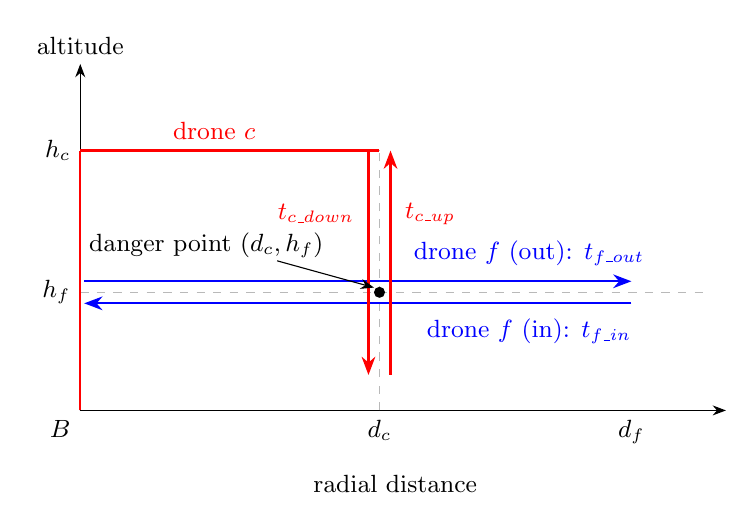
\begin{tikzpicture}[>=Stealth, font=\small]
        % axes
        \draw[->] (0,0) -- (8.2,0);
        \node[below] at (4.0,-0.7) {radial distance};
        \draw[->] (0,0) -- (0,4.4) node[above] {altitude};
        \node[below left] at (0,0) {$B$};

        % guide lines
        \draw[dashed,gray!55] (0,1.5) -- (8,1.5);
        \node[left] at (0,1.5) {$h_f$};
        \draw[dashed,gray!55] (0,3.3) -- (3.8,3.3);
        \node[left] at (0,3.3) {$h_c$};
        \draw[dashed,gray!55] (3.8,0) -- (3.8,3.3);
        \node[below] at (3.8,0) {$d_c$};
        \node[below] at (7,0) {$d_f$};

        % drone f : cruise at h_f, outbound (upper) and inbound (lower)
        \draw[thick,blue] (0,0) -- (0,1.5);
        \draw[thick,blue,->] (0.05,1.64) -- (7,1.64);
        \draw[thick,blue,->] (7,1.36) -- (0.05,1.36);
        \node[blue] at (5.7,2.0) {drone $f$ (out): $t_{f\_out}$};
        \node[blue] at (5.7,1.0) {drone $f$ (in): $t_{f\_in}$};

        % drone c : ascend, cruise to d_c, descend (left) and ascend (right) at d_c
        \draw[thick,red] (0,0) -- (0,3.3);
        \draw[thick,red] (0,3.3) -- (3.8,3.3);
        \draw[thick,red,->] (3.66,3.3) -- (3.66,0.45);
        \draw[thick,red,->] (3.94,0.45) -- (3.94,3.3);
        \node[red] at (1.7,3.55) {drone $c$};
        \node[red,left]  at (3.6,2.5) {$t_{c\_down}$};
        \node[red,right] at (4.0,2.5) {$t_{c\_up}$};

        % danger point
        \fill (3.8,1.5) circle (2pt);
        \node[align=center] at (1.6,2.1) {danger point $(d_c,h_f)$};
        \draw[->] (2.5,1.9) -- (3.73,1.56);
    \end{tikzpicture}
    \caption{Geometry of a vertical mid-air conflict in the distance--altitude plane. Drone $c$ serves a closer target ($d_c$) at a higher altitude ($h_c$) and crosses the lower cruise altitude $h_f$ while descending to and ascending from its delivery, at times $t_{c\_down}$ and $t_{c\_up}$. Drone $f$ serves a farther target at altitude $h_f$ and passes the radial distance $d_c$ outbound and inbound, at times $t_{f\_out}$ and $t_{f\_in}$. A conflict is flagged when any vertical and horizontal crossing time at the danger point $(d_c,h_f)$ fall within the safety buffer $t_{\mathit{safe}}$.}
    \label{fig:vertical_conflict}
\end{figure}

% To resolve the conflict without extending the mission makespan, the algorithm leverages Slack Absorption.
% It identifies which drone possesses the most idle time ($waitTime$) prior to its subsequent task (Line 21).
% A delay penalty $\Delta t$ is added to that drone's current ground waiting time (Line 22), mathematically forcing spatial separation. Crucially, this penalty is consecutively subtracted from the drone's future wait times (Line 23). 
% This localized absorption prevents the delay from cascading to the end of the schedule.
% Finally, the timeline is flagged, and the loops are broken (Lines 24--25) to trigger a complete timeline recalculation, guaranteeing that the shifted schedule does not precipitate secondary collisions elsewhere in the swarm.

% The conflict resolution algorithm is mathematically guaranteed to converge and avoid infinite loops. First, the applied delay penalty ($\Delta t$) is strictly positive, meaning that task start times are never pushed into the past. Second, absorbing this delay into existing slack simply reduces ground waiting times; it never pulls a future task backward on the mission clock. Finally, because there is a finite number of drone tasks but an infinite amount of available time, any repeated overlaps will eventually be pushed into empty, unoccupied time slots. Therefore, the schedule continuously moves toward a safe state, ensuring the algorithm always finishes in finite time. 

\begin{figure*}[!ht]
    \centering
    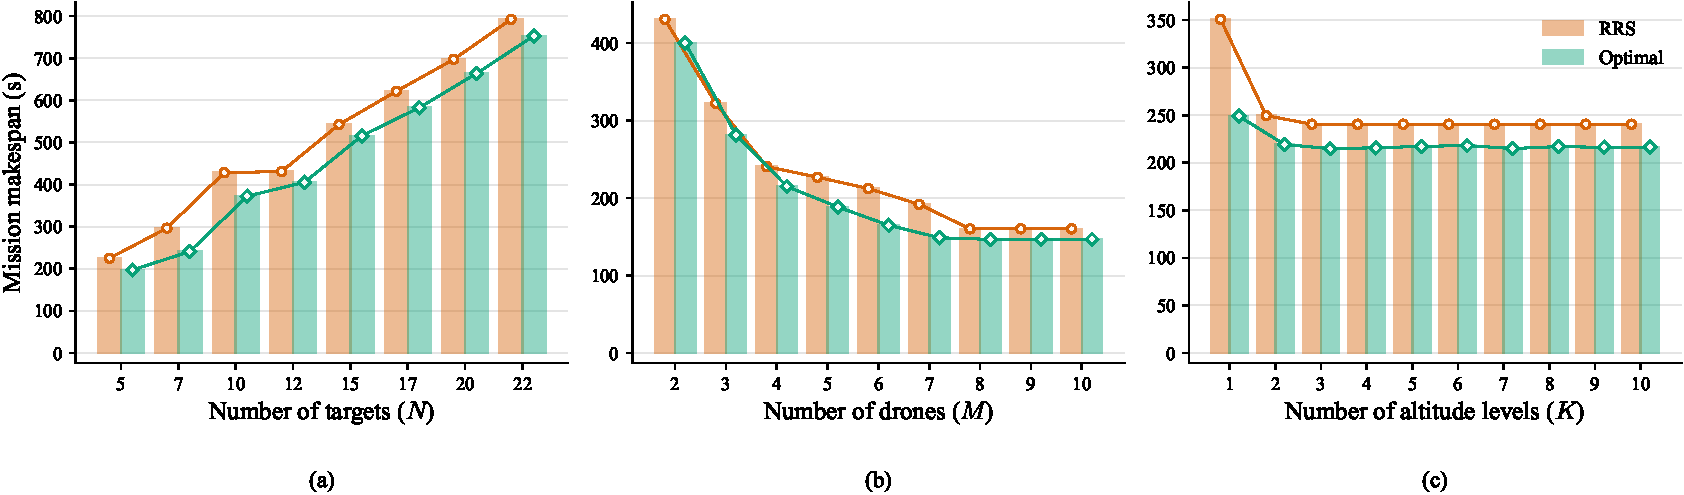
\includegraphics[width=\textwidth]{photos/makespan_RR1_opt.pdf}
    \caption{Mission makespan of RRS against the optimal MILP benchmark (grouped bars): (a) varying $N$ ($M=3$, $K=3$), (b) varying $M$ ($N=8$, $K=3$), and (c) varying $K$ ($N=8$, $M=4$). RRS tracks the optimum closely; the gap is widest at $K=1$, where a single altitude forces every sortie through one congested corridor.}
    \label{fig:makespan_rr1_opt}
\end{figure*}

\begin{figure*}[!ht]
    \centering
    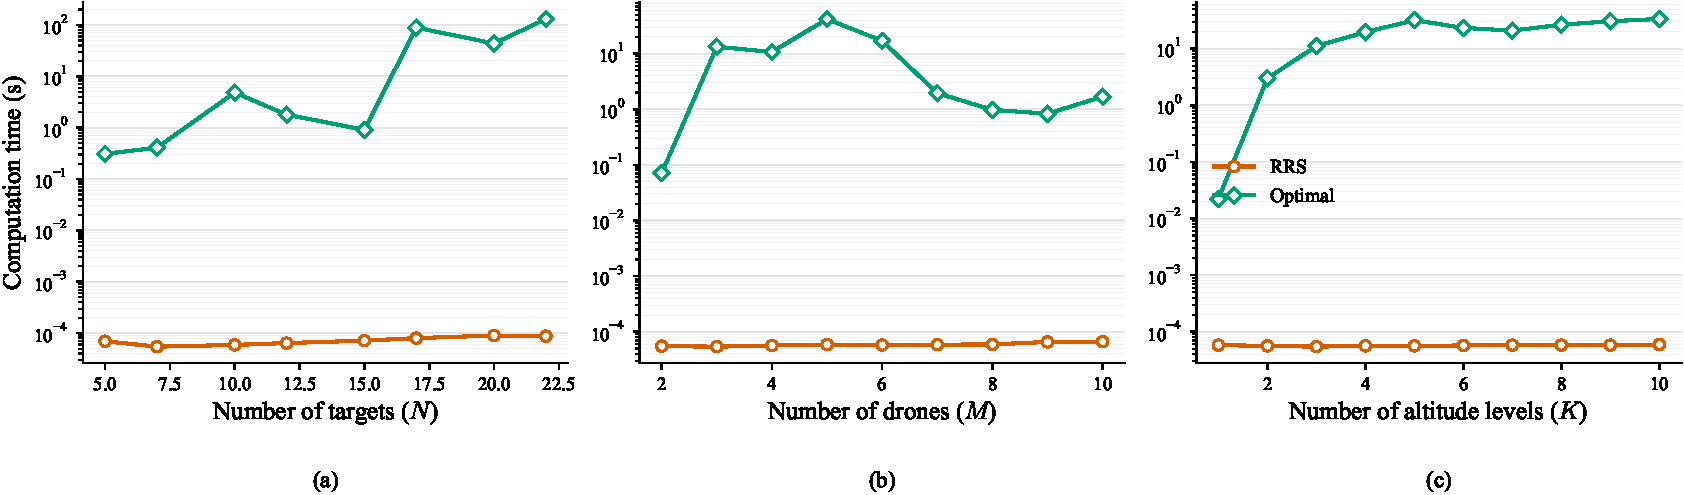
\includegraphics[width=\textwidth]{photos/computation_times_RR1_opt.pdf}
    \caption{Computation time of RRS against the optimal MILP benchmark (note the logarithmic vertical axis): (a) varying $N$ ($M=3$, $K=3$), (b) varying $M$ ($N=8$, $K=3$), and (c) varying $K$ ($N=8$, $M=4$). RRS runs in well under a millisecond, whereas the exact solver requires seconds to minutes and scales exponentially.}
    \label{fig:computaton_time_rr1_opt}
\end{figure*}



\begin{figure*}[!ht]
    \centering
    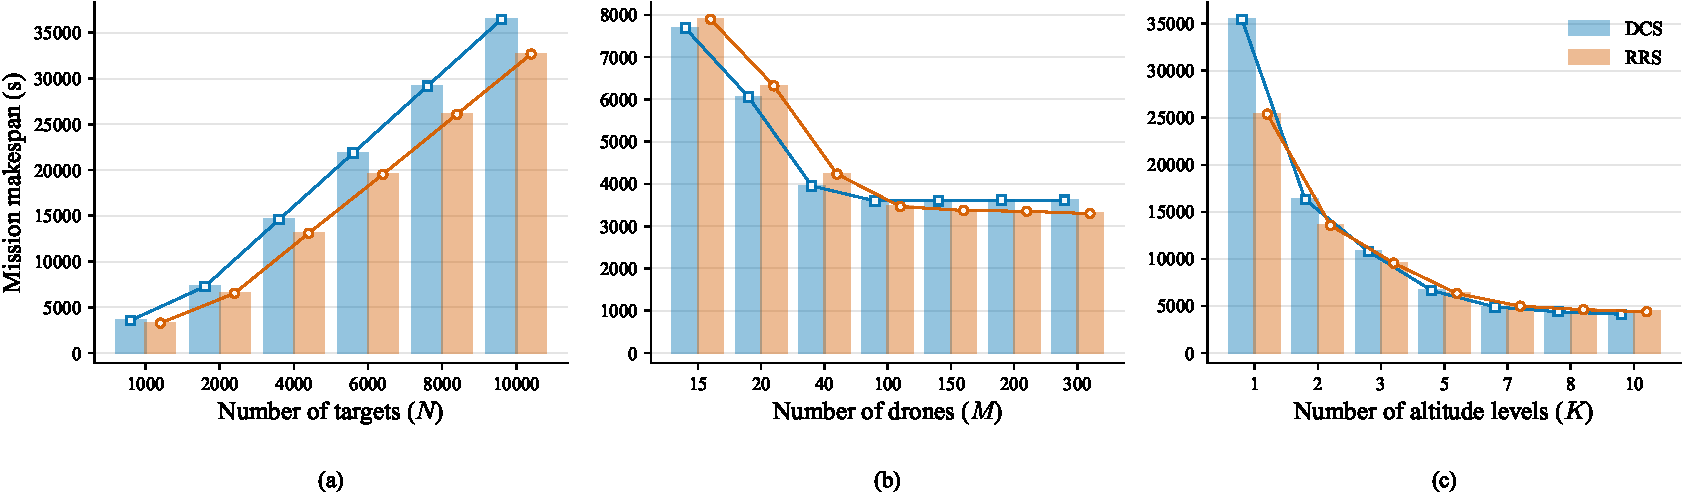
\includegraphics[width=\textwidth]{photos/makespan_heuristics.pdf}
    \caption{Mission makespan of DCS and RRS (grouped bars): (a) varying the number of targets $N$ ($M=400$, $K=10$), (b) varying the number of drones $M$ ($N=1000$, $K=10$), and (c) varying the number of altitude levels $K$ ($N=1000$, $M=40$).}
    \label{fig:makespan_heur}
\end{figure*}


\begin{figure*}[!ht]
    \centering
    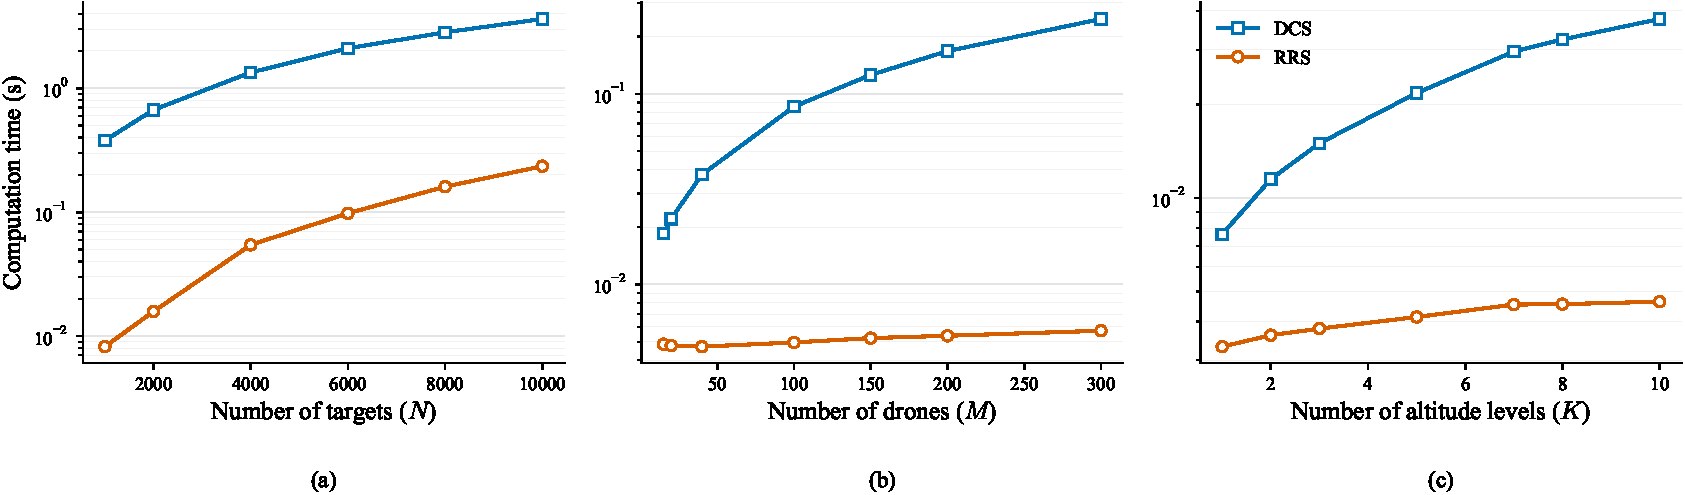
\includegraphics[width=\textwidth]{photos/computation_times_heuristics.pdf}
    \caption{Computation time of DCS and RRS (note the logarithmic vertical axis): (a) varying the number of targets $N$ ($M=400$, $K=10$), (b) varying the number of drones $M$ ($N=1000$, $K=10$), and (c) varying the number of altitude levels $K$ ($N=1000$, $M=40$). RRS is essentially independent of the fleet size $M$ (panel~b), reflecting its $O(NK)$ per-instance cost versus the $O(NMK)$ cost of DCS.}
    \label{fig:comptime_heur}
\end{figure*}




\begin{figure*}[!ht]   
    \centering
    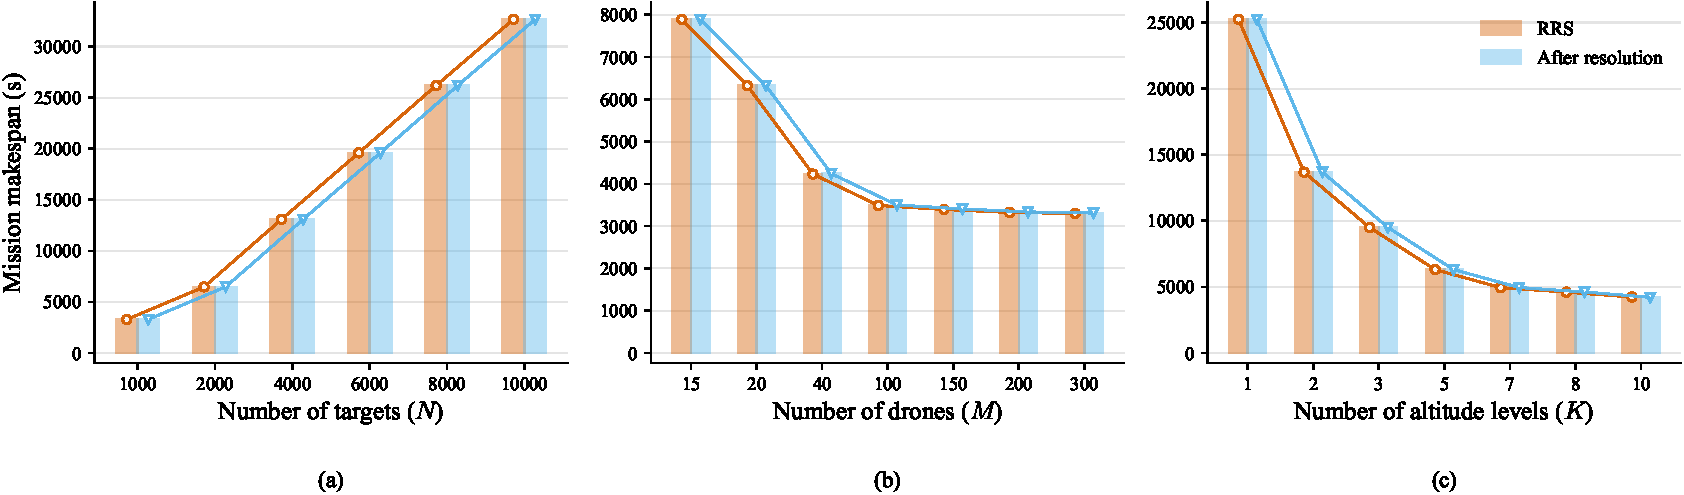
\includegraphics[width=\textwidth]{photos/makespan_RR1_res.pdf}
    \caption{Mission makespan of the baseline RRS schedule versus the schedule after conflict resolution: (a) varying $N$ ($M=400$, $K=10$), (b) varying $M$ ($N=1000$, $K=10$), and (c) varying $K$ ($N=1000$, $M=40$). The two bars in each group are virtually identical, confirming that the resolution layer preserves the optimized makespan.}
    \label{fig:makespan_rr1_res}
\end{figure*}     

\begin{figure*}[!ht]
    \centering
    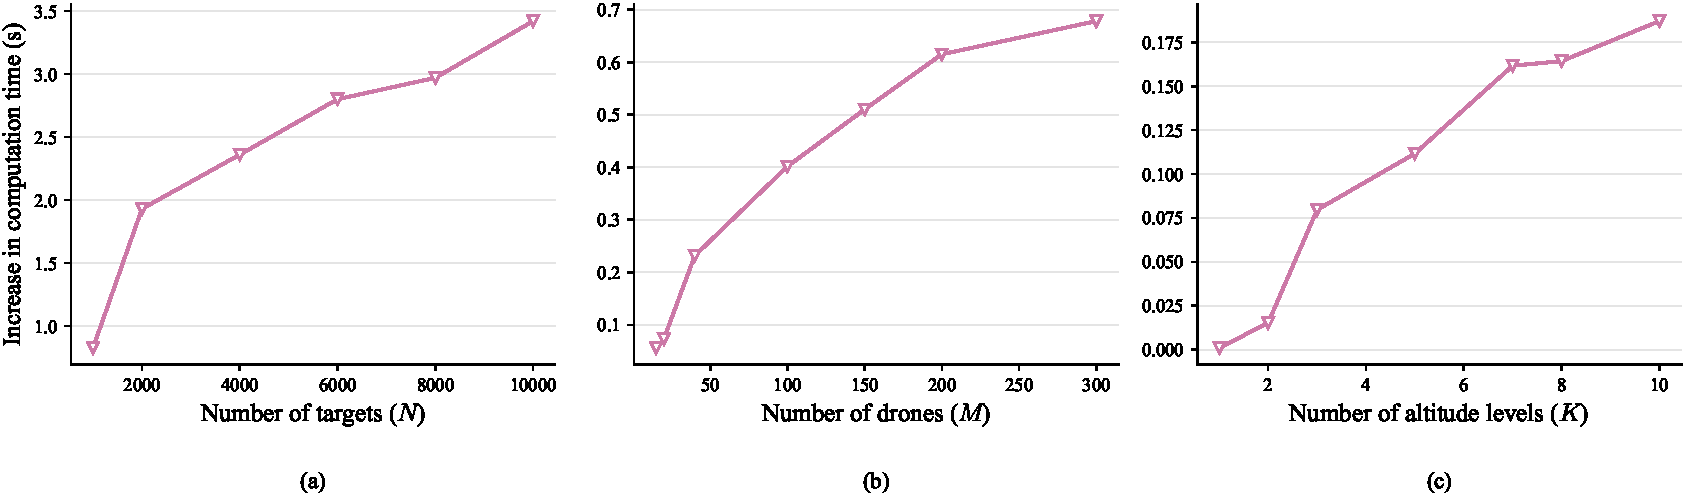
\includegraphics[width=\textwidth]{photos/computation_times_RR1_res.pdf}
    \caption{Increase in planning time introduced by the conflict-resolution layer (the additional time added on top of the baseline RRS schedule): (a) varying $N$ ($M=400$, $K=10$), (b) varying $M$ ($N=1000$, $K=10$), and (c) varying $K$ ($N=1000$, $M=40$).}
    \label{fig:computation_time_rr1_res}
\end{figure*}



\section{Performance Evaluation}

We evaluate the proposed algorithms for the mine dispensing problem within a two-dimensional Cartesian space, where the base is fixed at coordinates \([0, 0]\). 
The simulation environment models a battlefield of size \(300\,\text{m} \times 300\,\text{m}\).
The vertical and horizontal motion profiles of each drone are parameterized by an ascent/descent speed of \(2\,\text{m/s}\) and a cruise speed of \(5\,\text{m/s}\), respectively. The number of target sites is determined by the mine density \(\rho\) (in mines/m\(^2\)), which controls the spatial distribution of deployment locations. 
The proposed algorithms were implemented in MATLAB on a standard laptop with an AMD Ryzen~7 6000-series CPU and 16\,GB of RAM.

\subsection{Validation Against the Optimal MILP Solution}
As a first step, we validate the heuristics by comparing their solutions against the exact optimum obtained from the MILP formulation of Section~\ref{sec:optform}, solved in MATLAB with \texttt{intlinprog}.
Since the MILP is NP-hard, its optimal solution can only be computed for smaller-scale instances; we therefore benchmark against the exact solution over moderate values of \(N\), \(M\), and \(K\). On these small instances DCS and RRS achieve comparable makespan, so for clarity we report only the RRS--optimal comparison here and defer the DCS--RRS comparison to the scalability study below. The three sweeps are:


\begin{enumerate}
    \item makespan and computation time for varying \(N\), with \(M=3\) and \(K=3\);
    \item makespan and computation time for varying \(M\), with \(N=8\) and \(K=3\);
    \item makespan and computation time for varying \(K\), with \(N=8\) and \(M=4\).
\end{enumerate}


Figure~\ref{fig:makespan_rr1_opt} and Figure~\ref{fig:computaton_time_rr1_opt} report the makespan and computation-time comparisons, respectively.
RRS attains near-optimal makespan across all three sweeps while running in well under a millisecond, whereas the exact solver requires seconds to minutes and scales exponentially; RRS is thus a faithful and highly efficient surrogate for the exact solver. The gap is widest at \(K=1\), where a single altitude concentrates every sortie in one congested corridor.


\subsection{Comparison of Heuristic Algorithms}

Having validated RRS against the exact optimum, we next compare the two heuristics, Descending Cost Scheduling (DCS) and Round-Robin Scheduling (RRS), on large-scale instances beyond the reach of the MILP, in terms of both mission makespan and computational efficiency. Scalability is assessed across three problem dimensions:


\begin{enumerate}
    \item \textbf{Varying number of targets (\(N\))}: makespan (Figure~\ref{fig:makespan_heur}(a)) and computation time (Figure~\ref{fig:comptime_heur}(a)), with \(M=400\) and \(K=10\).
    \item \textbf{Varying number of drones (\(M\))}: makespan (Figure~\ref{fig:makespan_heur}(b)) and computation time (Figure~\ref{fig:comptime_heur}(b)), with \(N=1000\) and \(K=10\).
    \item \textbf{Varying altitude levels (\(K\))}: makespan (Figure~\ref{fig:makespan_heur}(c)) and computation time (Figure~\ref{fig:comptime_heur}(c)), with \(N=1000\) and \(M=40\).
\end{enumerate}

The results show that RRS attains a lower makespan than DCS as the number of targets grows (Figure~\ref{fig:makespan_heur}(a)) and remains comparable across the drone- and altitude-count sweeps, while being substantially cheaper to compute. DCS performs an exhaustive per-target search over all drones and altitudes, so its computation time is markedly higher (Figure~\ref{fig:comptime_heur}); its greedy approach also leave it with a larger makespan at the largest target counts. Overall, RRS achieves the best balance between mission efficiency and computational tractability, and is adopted as the heuristic of choice in the remainder of the paper.

\subsection{Scalability and Impact of the Conflict Resolution Layer}

To evaluate the operational impact of the proposed safety layer, we compared baseline RRS schedules with fully deconflicted schedules (``After Resolution'').
Unlike the MILP benchmark, which is constrained to moderate-sized instances, this evaluation was conducted on massive-scale swarm scenarios to stress-test the slack absorption and spatial hashing mechanisms.
Safety time buffer $t_{\mathit{safe}}$, angle tolerance $\theta_{\mathit{tol}}$, and delay penalty $\Delta t$ were set to 3 seconds, 2 degrees, and 5 seconds, respectively. 
Accordingly, Monte Carlo simulations were conducted across three primary configurations:

\begin{enumerate}
    \item Makespan and computation time comparison for baseline RRS and the resolved schedules with varying target counts \(N \in [1000, 10000]\), keeping fleet size \(M=400\) and altitudes \(K=10\).
    \item Makespan and computation time comparison for varying \(M \in [15, 300]\), keeping \(N=1000\) and \(K=10\).
    \item Makespan and computation time comparison for varying \(K \in [1, 10]\), keeping \(N=1000\) and \(M=40\).
\end{enumerate}


Figure~\ref{fig:makespan_rr1_res} compares the baseline and resolved makespans as grouped bars.
The two bars in each group are virtually identical, visually confirming that the resolution layer strictly preserves the optimized mission time.
Quantitatively, the conflict resolution layer increases the average mission makespan by a negligible margin---for instance, in the most extreme density scenario (\(N=10000\)), the makespan increases by an average of only 4 seconds on a 32,657-second mission (an increase of less than $0.02\%$). 
This effectively demonstrates the core advantage of the slack absorption strategy: necessary vertical intersection delays are successfully mathematically hidden within existing ground-wait times.

Figure~\ref{fig:computation_time_rr1_res} plots the additional computation time introduced by the safety layer, i.e. the increase in total planning time on top of the baseline RRS schedule.
While calculating continuous spatial-temporal overlaps across thousands of flight paths is inherently demanding, the implemented spatial hashing and time-bounding optimizations successfully avoid the quadratic $\mathcal{O}(N^2)$ growth of a naive pairwise check.
For the densest tested instance (\(N=10000\)), the baseline RRS algorithm executes in approximately $0.26$ seconds, while the complete post-processing resolution layer requires only an additional $3.42$ seconds. 
This confirms that the proposed safety architecture scales exceptionally well, remaining well within operational bounds for rapid, large-scale pre-flight mission planning.

% \subsection{Comparison of Heuristic Algorithms}

% The performance of the three heuristic algorithms—Descending Cost Scheduling (DCR), Round-Robin Scheduling  (RRS), and Flexible Round Robin Scheduling  (FRRS)—is analyzed in terms of both mission completion time (makespan) and computational efficiency. The following experiments were conducted to assess scalability across varying problem dimensions:



\section{Simulation Architecture in ROS2}

\begin{figure*}[!ht]
    \centering
    \resizebox{0.82\textwidth}{!}{%
    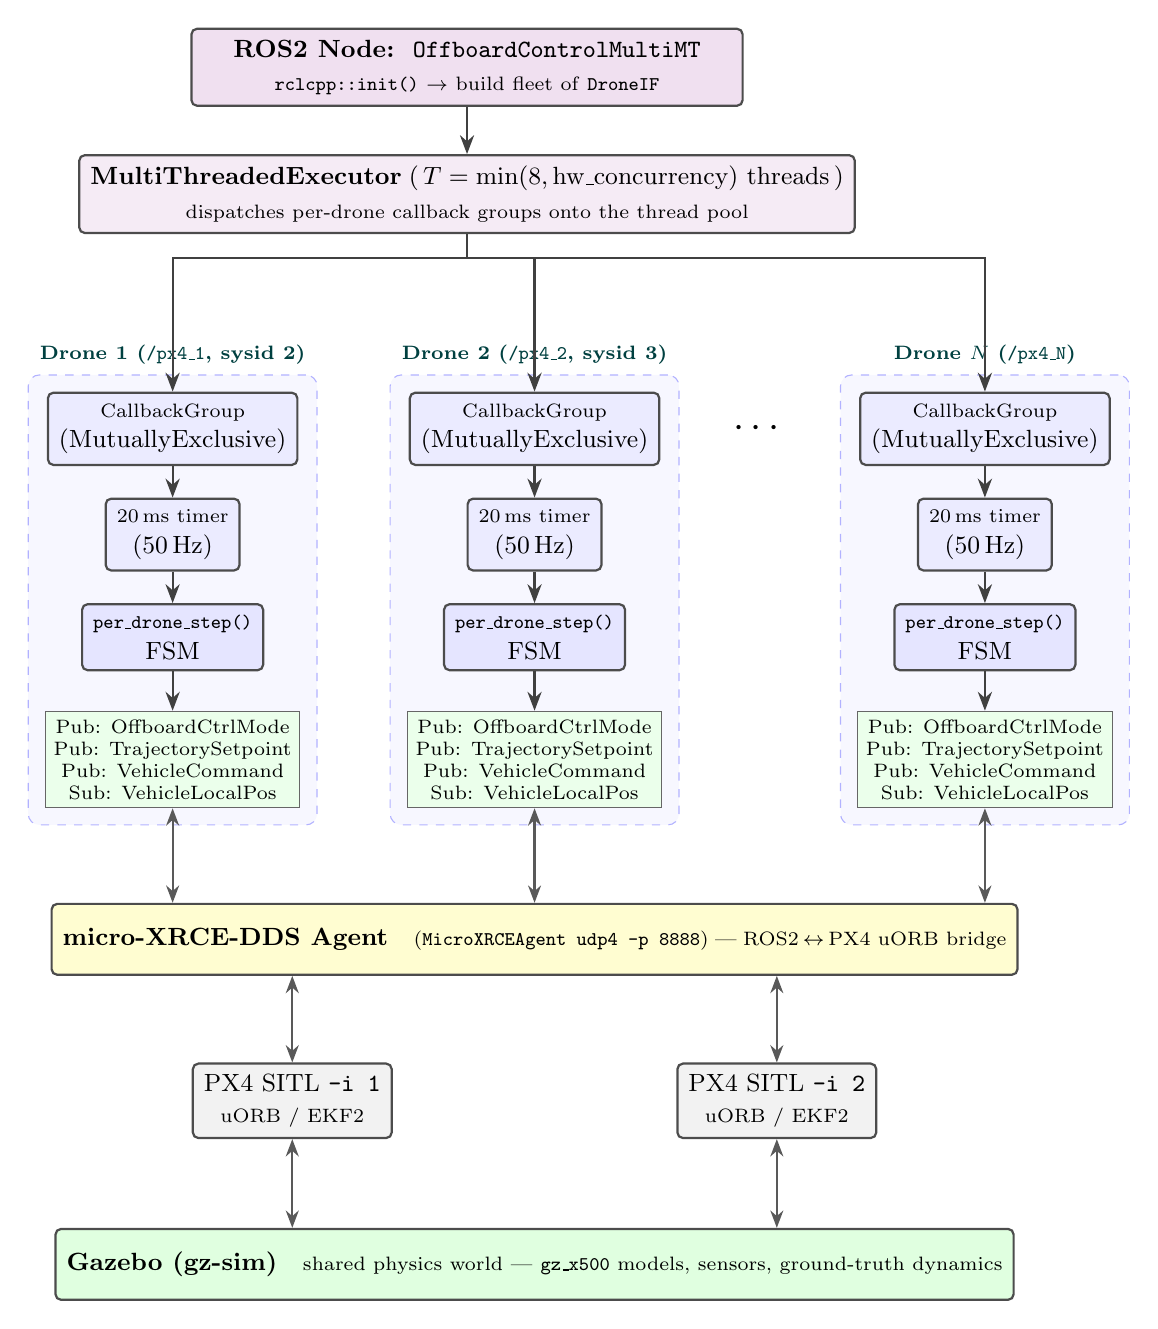
\begin{tikzpicture}[node distance=6mm and 10mm]

      \node[proc, fill=violet!12, minimum width=70mm] (node)
           {\textbf{ROS2 Node:}\; \texttt{OffboardControlMultiMT}\\[1pt]
            \scriptsize \texttt{rclcpp::init()} $\rightarrow$ build fleet of \texttt{DroneIF}};
      \node[proc, below=of node, minimum width=70mm, fill=violet!8] (exec)
           {\textbf{MultiThreadedExecutor}\;(\,$T=\min(8,\text{hw\_concurrency})$ threads\,)\\[1pt]
            \scriptsize dispatches per-drone callback groups onto the thread pool};
      \draw[flow] (node) -- (exec);

      \node[proc, anchor=north, fill=blue!8] (cg1) at ($(exec.south west)+(12mm,-20mm)$)
           {\scriptsize CallbackGroup\\(MutuallyExclusive)};
      \node[proc, below=4mm of cg1, fill=blue!8] (t1) {\scriptsize 20\,ms timer\\(50\,Hz)};
      \node[proc, below=4mm of t1, fill=blue!10] (s1) {\scriptsize \texttt{per\_drone\_step()}\\ FSM};
      \node[io, below=5mm of s1] (io1)
           {Pub: OffboardCtrlMode\\Pub: TrajectorySetpoint\\Pub: VehicleCommand\\Sub: VehicleLocalPos};

      \node[proc, right=14mm of cg1, fill=blue!8] (cg2) {\scriptsize CallbackGroup\\(MutuallyExclusive)};
      \node[proc, below=4mm of cg2, fill=blue!8] (t2) {\scriptsize 20\,ms timer\\(50\,Hz)};
      \node[proc, below=4mm of t2, fill=blue!10] (s2) {\scriptsize \texttt{per\_drone\_step()}\\ FSM};
      \node[io, below=5mm of s2] (io2)
           {Pub: OffboardCtrlMode\\Pub: TrajectorySetpoint\\Pub: VehicleCommand\\Sub: VehicleLocalPos};

      \node[right=8mm of cg2, font=\Large\bfseries] (dots) {$\cdots$};
      \node[proc, right=8mm of dots, fill=blue!8] (cgN) {\scriptsize CallbackGroup\\(MutuallyExclusive)};
      \node[proc, below=4mm of cgN, fill=blue!8] (tN) {\scriptsize 20\,ms timer\\(50\,Hz)};
      \node[proc, below=4mm of tN, fill=blue!10] (sN) {\scriptsize \texttt{per\_drone\_step()}\\ FSM};
      \node[io, below=5mm of sN] (ioN)
           {Pub: OffboardCtrlMode\\Pub: TrajectorySetpoint\\Pub: VehicleCommand\\Sub: VehicleLocalPos};

      \draw[flow] (cg1) -- (t1); \draw[flow] (t1) -- (s1); \draw[flow] (s1) -- (io1);
      \draw[flow] (cg2) -- (t2); \draw[flow] (t2) -- (s2); \draw[flow] (s2) -- (io2);
      \draw[flow] (cgN) -- (tN); \draw[flow] (tN) -- (sN); \draw[flow] (sN) -- (ioN);

      \draw[flow] (exec.south) -- ++(0,-3mm) -| (cg1);
      \draw[flow] (exec.south) -- ++(0,-3mm) -| (cg2);
      \draw[flow] (exec.south) -- ++(0,-3mm) -| (cgN);

      \begin{scope}[on background layer]
        \node[lane, fit=(cg1)(io1), label={[font=\scriptsize\bfseries,teal!50!black]above:Drone 1 (\texttt{/px4\_1}, sysid 2)}] {};
        \node[lane, fit=(cg2)(io2), label={[font=\scriptsize\bfseries,teal!50!black]above:Drone 2 (\texttt{/px4\_2}, sysid 3)}] {};
        \node[lane, fit=(cgN)(ioN), label={[font=\scriptsize\bfseries,teal!50!black]above:Drone $N$ (\texttt{/px4\_N})}] {};
      \end{scope}

      \node[ext, fill=yellow!18, below=12mm of io2, minimum width=120mm] (dds)
           {\textbf{micro-XRCE-DDS Agent}\quad\scriptsize(\texttt{MicroXRCEAgent udp4 -p 8888})\;---\;ROS2\,$\leftrightarrow$\,PX4 uORB bridge};
      \draw[bus] (io1) -- (io1|-dds.north);
      \draw[bus] (io2) -- (dds.north);
      \draw[bus] (ioN) -- (ioN|-dds.north);

      \node[ext, below left=11mm and 18mm of dds.south, fill=gray!10] (px1) {PX4 SITL \texttt{-i 1}\\\scriptsize uORB / EKF2};
      \node[ext, below right=11mm and 18mm of dds.south, fill=gray!10] (px2) {PX4 SITL \texttt{-i 2}\\\scriptsize uORB / EKF2};
      \draw[bus] (px1.north) -- (px1.north|-dds.south);
      \draw[bus] (px2.north) -- (px2.north|-dds.south);

      \node[ext, below=32mm of dds, fill=green!12, minimum width=120mm] (gz)
           {\textbf{Gazebo (gz-sim)}\quad\scriptsize shared physics world ---
            \texttt{gz\_x500} models, sensors, ground-truth dynamics};
      \draw[bus] (px1.south) -- (px1.south|-gz.north);
      \draw[bus] (px2.south) -- (px2.south|-gz.north);

    \end{tikzpicture}}
    \caption{Concurrent ROS\,2--PX4 software-in-the-loop architecture. A single \texttt{OffboardControlMultiMT} node flies the whole fleet: each vehicle owns an independent \texttt{DroneIF} interface and a mutually-exclusive callback group, all serviced in parallel by one \texttt{MultiThreadedExecutor}. Per-drone publishers and subscribers are bridged to the corresponding PX4 SITL instance through the micro-XRCE-DDS agent, and every instance shares a single Gazebo world.}
    \label{fig:ROS2_arch}
\end{figure*}

To demonstrate that the schedules generated by the proposed DCS and RRS algorithms---together with the slack-absorption deconfliction layer---are executable on a realistic flight stack, we developed a \emph{software-in-the-loop} (SITL) simulation. In an SITL simulation, the same autopilot software that would run on a real drone runs unmodified on an ordinary computer, so a planned mission can be executed and observed just as it would be in flight, but with no physical vehicle. The pipeline is built on three widely used open-source tools: \emph{PX4}, the autopilot that stabilizes and flies each quadrotor; \emph{Gazebo}, a 3-D physics simulator that supplies the virtual world, the vehicle dynamics, and the sensors; and \emph{ROS\,2} (Robot Operating System~2), the middleware through which our mission software exchanges messages with each PX4 autopilot. Several PX4-controlled quadrotors fly simultaneously within a single shared Gazebo world. The overall architecture is summarized in Fig.~\ref{fig:ROS2_arch}, and the mission logic executed for each vehicle is detailed in Fig.~\ref{fig:ROS2_fsm}.

The governing design requirement is \emph{genuine concurrency}. Throughout this section, the \emph{controller} refers to our own mission software---a single program that decides where each drone should go and streams those commands to the PX4 autopilots. It should not be confused with PX4's onboard flight controller, which stabilizes each individual vehicle; our controller sits above PX4 and coordinates the fleet. Because the optimized makespan is defined under the assumption that all vehicles execute their assigned missions simultaneously, the controller must issue and service every drone's commands within the same control cycle. If it instead stepped through the drones one after another in a single sequence, the command sent to the last drone in a cycle would lag that of the first, and at large fleet sizes this accumulated delay would distort the very temporal profile that the optimization layer assumes. The architecture described below is engineered to preserve this simultaneity when transferring an abstract schedule onto an embodied multi-vehicle simulation.

\subsection{Concurrent execution model}

A few ROS\,2 concepts are needed to explain the design. A \emph{node} is a single program within the system. The work a node performs is organized into \emph{callbacks}---short functions that run in response to an event, such as a periodic timer firing or a new sensor message arriving. An \emph{executor} is the part of ROS\,2 that decides when to run these callbacks: a single-threaded executor runs them strictly one at a time, whereas a \emph{multi-threaded executor} owns a pool of \emph{worker threads} (independent streams of execution that the operating system can place on separate CPU cores) and can therefore run several callbacks at the same instant.

Our controller is a single node, \texttt{OffboardControlMultiMT}, that creates one self-contained interface object per drone---holding that drone's message channels, its timer, and its mission state---and registers them all with one multi-threaded executor. The design hinges on how the callbacks are grouped. Each drone is placed in its own \emph{mutually-exclusive callback group}: a group whose member callbacks are never allowed to run at the same time. This restriction is deliberate. Within a single drone, the timer callback (which advances that drone's mission logic) and the sensor callback (which stores its latest position) both read and write the \emph{same} variables; were they to run simultaneously on two threads, they could interleave and corrupt each other's data---a fault known as a \emph{race condition}. Confining each drone to a mutually-exclusive group makes such overlaps impossible. Crucially, the restriction applies only \emph{within} a drone: callbacks belonging to \emph{different} drones lie in different groups and are free to run in parallel on different threads. The result is exactly the behavior required---all drones advance together, yet each drone's internal state stays consistent.

Because two callbacks of the same drone can never overlap, that drone's state (its mission stage, latest position, and active target) is updated safely without any \emph{locks}---the usual, and comparatively slow, software mechanism for guarding data shared between threads. This ``race-free and lock-free by construction'' property is what lets a single computer drive an entire fleet both \emph{correctly} (no corrupted state) and \emph{efficiently} (no locking overhead). The worker pool is sized to $\min(8,\text{ number of CPU cores})$. This number bounds only how many drones execute at literally the same instant; it does not limit how many drones can be simulated---additional drones simply share the pool and run concurrently in a rapidly time-sliced fashion. On a typical multi-core machine this comfortably flies fleets large enough to exercise the planned schedules.

It is worth being explicit about \emph{why} a single multi-threaded program is the appropriate choice \emph{for this validation}, as opposed to the more deployment-like alternative of running one separate control program per drone that communicate over a network. In the mine-dispensing mission, all coordination is decided in advance by the offline scheduler; each drone then flies a fixed, pre-assigned set of sorties and never needs to communicate with the other drones while in flight. Splitting the controller into many separate programs would therefore add the overhead and complexity of inter-program communication without exercising any capability that this problem actually requires. The single-program design instead provides two things that directly serve validation. First, every drone is driven from one common clock, so the vehicles genuinely start and advance together---the simultaneity that the makespan assumes. Second, because all vehicles report into the same program, their positions and timestamps are recorded on a single, already-aligned timeline; this makes it straightforward to verify afterwards, at the level of the whole mission, both the achieved makespan and that no two drones ever violated their sector--altitude separation. We stress that this is a deliberate choice for \emph{simulation and validation on a single machine}. A real deployment naturally places one small companion computer on each drone---one program per vehicle---and the per-drone interface object used here maps directly onto that arrangement.

\subsection{System initialization and mission configuration}

On startup the node builds the fleet from a compact per-vehicle configuration. For each drone this specifies its \emph{namespace} (a unique name prefix, such as \texttt{/px4\_1} or \texttt{/px4\_2}, that keeps each drone's messages separate from the others'), a numeric identifier used by PX4 ($\text{MAV\_SYS\_ID}$), the target coordinates and cruise altitude taken from the optimized assignment, and a start delay. The start delay is the mechanism by which the temporal output of the scheduling layer is injected into the simulation: the staggered release times and ground-wait (slack) intervals produced by the deconfliction stage are encoded directly as each vehicle's activation offset, so that the simulated fleet reproduces the optimized launch sequence rather than releasing every drone at once.

\subsection{Communication interface and PX4 bridge}

ROS\,2 programs communicate by passing messages over named channels called \emph{topics}: a \emph{publisher} sends messages on a topic and a \emph{subscriber} receives them. For every vehicle the controller creates three publishers and one subscriber. The publishers send \texttt{OffboardControlMode} (which informs PX4 that an external program is taking over position control), \texttt{TrajectorySetpoint} (the commanded target position), and \texttt{VehicleCommand} (mode changes, arming, and landing). Target positions are expressed in the local \emph{NED} frame---a standard aviation convention in which the three axes point North, East, and Down, so that a negative vertical coordinate corresponds to altitude above the ground. The subscriber receives \texttt{VehicleLocalPosition}, the drone's estimated position produced by PX4's onboard state estimator, \emph{EKF2} (an Extended Kalman Filter that fuses the inertial, satellite-navigation, and barometric sensors into a single best estimate of the vehicle's position); the controller uses this estimate to judge when a drone has reached its current waypoint.

The link between our ROS\,2 controller and each PX4 autopilot is provided by the \emph{micro-XRCE-DDS} agent~\cite{eProsimaMicroXRCEDDS}, the standard component PX4 uses for this purpose: it translates PX4's internal messages into the format ROS\,2 understands, and vice versa. Because all simulated drones share one world and one common message space, each command must be addressed to the correct vehicle; this is done by stamping every \texttt{VehicleCommand} with the target drone's identifier ($\text{MAV\_SYS\_ID}$), so that only the intended airframe acts on it.

\subsection{Per-drone control loop and finite-state machine}

\begin{figure*}[!ht]
    \centering
    \resizebox{0.78\textwidth}{!}{%
    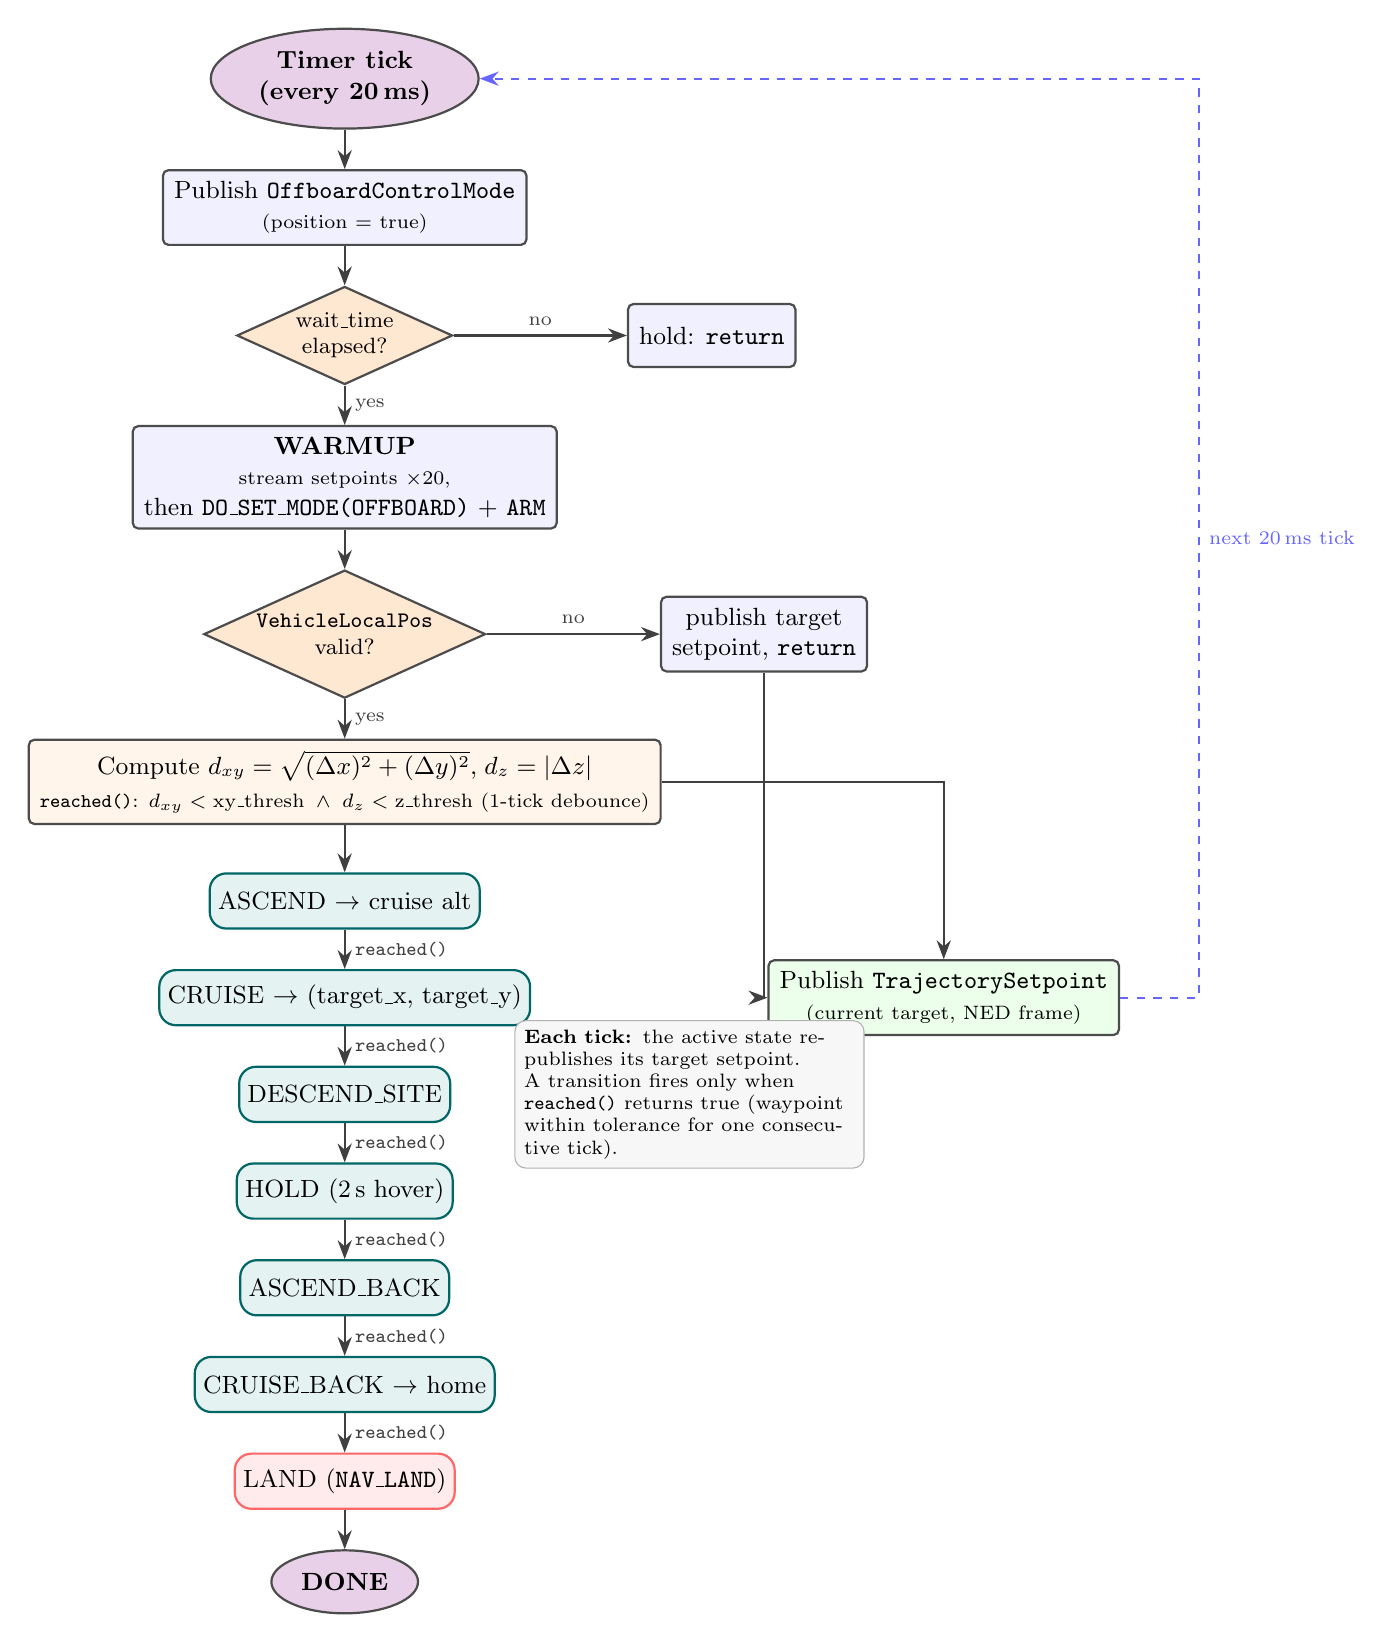
\begin{tikzpicture}[node distance=5mm and 14mm]

      \node[term] (tick) {Timer tick\\(every 20\,ms)};
      \node[proc, below=of tick] (ofb) {Publish \texttt{OffboardControlMode}\\\scriptsize(position = true)};
      \node[dec, below=of ofb] (waited) {wait\_time\\elapsed?};
      \node[proc, right=22mm of waited] (hold0) {hold: \texttt{return}};
      \node[proc, below=of waited] (warm)
           {\textbf{WARMUP}\\\scriptsize stream setpoints $\times 20$,\\ then \texttt{DO\_SET\_MODE(OFFBOARD)} + \texttt{ARM}};
      \node[dec, below=of warm] (posval) {\texttt{VehicleLocalPos}\\valid?};
      \node[proc, right=22mm of posval] (hold1) {publish target\\setpoint, \texttt{return}};

      \node[proc, below=of posval, fill=orange!8] (dist)
           {Compute $d_{xy}=\sqrt{(\Delta x)^2+(\Delta y)^2}$,\;$d_z=|\Delta z|$\\[1pt]
            \scriptsize \texttt{reached()}: $d_{xy}<\text{xy\_thresh}\;\wedge\;d_z<\text{z\_thresh}$ (1-tick debounce)};

      \node[state, below=6mm of dist] (sasc)   {ASCEND $\rightarrow$ cruise alt};
      \node[state, below=of sasc]     (scru)   {CRUISE $\rightarrow$ (target\_x, target\_y)};
      \node[state, below=of scru]     (sdes)   {DESCEND\_SITE};
      \node[state, below=of sdes]     (shold)  {HOLD (2\,s hover)};
      \node[state, below=of shold]    (sascb)  {ASCEND\_BACK};
      \node[state, below=of sascb]    (scrub)  {CRUISE\_BACK $\rightarrow$ home};
      \node[state, below=of scrub, fill=red!8, draw=red!60] (sland) {LAND (\texttt{NAV\_LAND})};
      \node[term, below=of sland] (done) {DONE};

      \node[proc, right=30mm of scru, fill=green!8] (pubsp)
           {Publish \texttt{TrajectorySetpoint}\\\scriptsize (current target, NED frame)};

      \draw[flow] (tick) -- (ofb);
      \draw[flow] (ofb) -- (waited);
      \draw[flow] (waited) -- node[above,font=\scriptsize]{no} (hold0);
      \draw[flow] (waited) -- node[right,font=\scriptsize]{yes} (warm);
      \draw[flow] (warm) -- (posval);
      \draw[flow] (posval) -- node[above,font=\scriptsize]{no} (hold1);
      \draw[flow] (posval) -- node[right,font=\scriptsize]{yes} (dist);
      \draw[flow] (dist) -- (sasc);

      \foreach \a/\b in {sasc/scru, scru/sdes, sdes/shold, shold/sascb, sascb/scrub, scrub/sland} {
        \draw[flow] (\a) -- node[right,font=\scriptsize]{\texttt{reached()}} (\b);
      }
      \draw[flow] (sland) -- (done);

      \draw[flow] (dist.east) -| (pubsp);
      \draw[flow] (hold1) |- (pubsp);
      \draw[flow, dashed, blue!60] (pubsp.east) -- ++(10mm,0)
            |- node[pos=0.25,right,font=\scriptsize,blue!60]{next 20\,ms tick} (tick.east);

      \node[font=\scriptsize, align=left, draw=black!30, fill=black!3, rounded corners,
            right=8mm of sdes, text width=42mm] (note)
           {\textbf{Each tick:} the active state re-publishes its target setpoint.
            A transition fires only when \texttt{reached()} returns true
            (waypoint within tolerance for one consecutive tick).};

    \end{tikzpicture}}
    \caption{Per-drone finite-state machine executed on every 20\,ms (50\,Hz) timer callback. Each vehicle runs an independent instance; a stage transition is triggered only by the debounced, position-based \texttt{reached()} check, while a continuous \texttt{TrajectorySetpoint} stream is maintained to retain offboard authority.}
    \label{fig:ROS2_fsm}
\end{figure*}

Each drone runs its own timer that fires every 20\,ms (50 times per second). On every firing the controller executes that drone's step function, which does two things. It first re-sends the \texttt{OffboardControlMode} message: PX4 accepts external commands only while they keep arriving, so this repeated message acts as a \emph{heartbeat} that must be refreshed continuously, or PX4 reverts to its own control. It then advances the drone's \emph{finite-state machine} (FSM)---a simple controller that is always in exactly one named ``state'' and moves to the next state when a defined condition is met. This mission FSM is entirely our own logic, layered on top of PX4; PX4 itself performs only the low-level flying (stabilization, position holding, and arming). The FSM proceeds through the following stages (Fig.~\ref{fig:ROS2_fsm}):
\begin{itemize}
  \item \textit{WAIT\_START:} idle until the configured activation delay has elapsed.
  \item \textit{WARMUP:} stream setpoints over a short warm-up window, then command \texttt{OFFBOARD} mode (\texttt{VEHICLE\_CMD\_DO\_SET\_MODE}) followed by \texttt{ARM}.
  \item \textit{ASCEND:} climb vertically to the assigned cruise altitude.
  \item \textit{CRUISE:} translate horizontally to the target coordinates.
  \item \textit{DESCEND\_SITE:} descend to the delivery altitude above the target.
  \item \textit{HOLD:} hover briefly at the delivery site (the payload-drop dwell).
  \item \textit{ASCEND\_BACK / CRUISE\_BACK:} climb back to cruise altitude and return to the launch position.
  \item \textit{LAND:} issue \texttt{VEHICLE\_CMD\_NAV\_LAND} and hold the final setpoint.
  \item \textit{DONE:} mission complete.
\end{itemize}
Because each vehicle owns a separate FSM instance and timer, the stages of different drones evolve independently and concurrently; a drone still warming up does not stall a drone already cruising.

\subsection{Closed-loop waypoint guidance}

Stage transitions are driven by position feedback rather than open-loop timing. On each tick the controller compares the active target $(x_t,y_t,z_t)$ against the latest estimate $(x,y,z)$ using the horizontal and vertical errors
\[ d_{xy}=\sqrt{(x_t-x)^2+(y_t-y)^2}, \qquad d_z=\lvert z_t-z\rvert .\]
A waypoint is deemed reached only when both $d_{xy}$ and $d_z$ fall below the tolerances \texttt{xy\_thresh} and \texttt{z\_thresh}; a one-cycle \emph{debounce} additionally requires this condition to hold on two consecutive timer firings before the FSM advances, which suppresses spurious transitions caused by momentary noise in the position estimate. A separate concern is \emph{overshoot}---a drone flying past its target and swinging back and forth about it. This is handled not by our logic but by PX4's underlying position controller, which is damped so that the vehicle decelerates smoothly onto the target and settles rather than oscillating; moreover, once the drone is inside the tolerance band the commanded target is held unchanged, so the vehicle comes to rest instead of repeatedly crossing the boundary. To ensure a drone actually registers as ``reached'' rather than hovering just outside it, the tolerances are set slightly larger than the controller's small residual steady-state error. Until a stage's condition is met---or while a valid position estimate is not yet available---the controller keeps re-sending the current target, both to guide the drone and because an uninterrupted stream of commands is itself required to remain in offboard mode.

\subsection{Summary}

In summary, the simulation framework couples the planning layer to a high-fidelity flight simulation through four properties that together make it a faithful test of dense-swarm schedules: (i) all drones are flown in genuine parallel, one mutually-exclusive callback group per vehicle on a shared multi-threaded executor; (ii) each drone's state is updated safely without locks, by construction; (iii) every drone is guided by our own 50\,Hz, feedback-driven mission FSM; and (iv) the optimized schedule---including its computed ground-wait (slack) times---is reproduced exactly through per-drone start offsets.

Figure~\ref{fig:gazebo_snapshots} shows the fleet executing an RRS-generated schedule in the Gazebo world, and a supplementary video\footnote{Supplementary video demonstrating the simultaneous multi-drone execution: \url{https://example.org/REPLACE-WITH-VIDEO-LINK}} records several drones flying their assigned sorties at the same time. This end-to-end execution on the PX4 flight stack confirms that the makespan and deconfliction results of the preceding sections carry over from the abstract schedule to a realistic, simultaneously-flying fleet.

\begin{figure}[!ht]
    \centering
    \IfFileExists{photos/gazebo_snapshots.png}{%
        \includegraphics[width=\columnwidth]{photos/gazebo_snapshots.png}%
    }{%
        \fbox{\parbox[c][4.2cm][c]{0.92\columnwidth}{\centering\itshape
        Placeholder --- replace with \texttt{photos/gazebo\_snapshots.png}: Gazebo
        snapshots of the fleet executing an RRS schedule (e.g.\ climbing to
        separated cruise altitudes, cruising toward targets, delivering, and
        returning to base).}}%
    }
    \caption{Snapshots of the software-in-the-loop execution: multiple PX4-controlled
    quadrotors flying an RRS-generated schedule simultaneously in a shared Gazebo world,
    each at its assigned cruise altitude.}
    \label{fig:gazebo_snapshots}
\end{figure}

\section{Conclusion and Future Work}


In this paper, we addressed the mine dispensing problem using a fleet of autonomous aerial vehicles operating over a defined battlefield. 
The problem was formulated as a mixed-integer optimization model and shown to be NP-hard, motivating the development of scalable heuristic algorithms.
Two scheduling algorithms—Descending Cost Scheduling (DCS) and Round-Robin Scheduling (RRS)—were proposed to efficiently allocate drones to targets while minimizing overall mission makespan and computation time.

Extensive simulations were performed in MATLAB to evaluate the performance of the proposed algorithms under varying numbers of drones, targets, and altitude levels. 
The results demonstrated that RRS consistently achieves near-optimal performance while maintaining significantly lower computational complexity, making it well-suited for large-scale mission scenarios.

Furthermore, a deterministic post-processing conflict-resolution layer was introduced to guarantee collision-free vertical flight-path transitions during dense swarm operations.
By leveraging spatial hashing and temporal slack absorption, the proposed architecture successfully resolved mid-air intersections while strictly preserving the optimized mission makespan. 
The evaluation confirmed that this safety layer scales exceptionally well, introducing a negligible makespan increase of less than 0.02\% and minimal computational overhead even in extreme scenarios containing up to 10,000 targets.

To validate the practical feasibility of the proposed approach, the scheduling framework was integrated into a ROS2-based architecture and tested in the Gazebo simulation environment. 
The end-to-end pipeline—from mission initialization to trajectory execution—confirmed that the algorithms can be effectively deployed in real-time drone coordination tasks.

Future work will extend this framework to handle dynamic task allocation, transitioning from static, pre-planned missions to environments where targets and constraints evolve in real time. 
To address the computational demands of real-time adaptability, we plan to explore learning-based methods, particularly Multi-Agent Reinforcement Learning (MARL) and Offline RL, to develop adaptive, highly responsive scheduling policies.
Additionally, integrating data-driven system identification approaches, such as Koopman operator theory and Sparse Identification of Nonlinear Dynamics (SINDy), will be investigated to more accurately model the complex, non-linear dynamics of the UAV swarm and environmental disturbances, further bridging the gap between simulation and real-world deployment.

\bibliographystyle{asmejour}

\bibliography{myreferences}

\end{document}
 
